\documentclass[draftspec]{sbmlpkgspec}

\newcommand{\fixttspace}{\hspace*{1pt}}

\newcommand{\sbmlthreedynamic}{SBML Level~3 Package Specification for Dynamic Structures, Version~1\xspace}
\newcommand{\sbmlthreecore}{SBML Level~3 Version~2 Core\xspace}

%To remove when validationrules.tex is modified
\newcommand{\Dimension}{\defRef{Dimension}{sec:dimension}\xspace}
\newcommand{\ListOfDimensions}{\defRef{ListOfDimensions}{sec:dimension}\xspace}
\newcommand{\Index}{\defRef{Index}{sec:index}\xspace}
\newcommand{\ListOfIndices}{\defRef{ListOfIndices}{sec:index}\xspace}

\newcommand{\SpatialComponent}{\defRef{SpatialComponent}{subsec:spatialComp}\xspace}
\newcommand{\ListOfSpatialComponents}{\defRef{ListOfSpatialComponents}{subsec:listSpatialComp}\xspace}
\newcommand{\Behavior}{\absDefRef{Behavior}{Behavior-class}}
\newcommand{\Behaviors}{\absDefRef{Behaviors}{Behavior-class}}

\newcommand{\Element}{\defRef{Element}{subsec:Element}\xspace}
\newcommand{\ListOfElements}{\defRef{ListOfElements}{subsec:ListOfElements}\xspace}

\newcommand{\ListofGroups}{\textbf{\class{ListofGroups}}\xspace}


\newcommand{\Compartments}{\textbf{\class{Compartments}}\xspace}
\newcommand{\Reactions}{\textbf{\class{Reactions}}\xspace}
\newcommand{\Parameters}{\textbf{\class{Parameters}}\xspace}
\newcommand{\ChangedMath}{\textbf{\class{ChangedMath}}\xspace}


\begin{document}

\packageTitle{Hierarchical Model Composition}
\packageVersion{Version 1 (Draft)}
\packageVersionDate{8 June 2012}
\packageGeneralURL{http://sbml.org/Documents/Specifications/Packages/Hierarchical_Model_Composition}
\packageThisVersionURL{http://sbml.org/Documents/Specifications/Packages/Hierarchical_Model_Composition/XXXXX}

\author{%
  \begin{tabular}{>{\hspace{20pt}}c>{\hspace{20pt}}c}
    Lucian P. Smith			& Michael Hucka\\ 
    \mailto{lpsmith@u.washington.edu}	& \mailto{mhucka@caltech.edu}\\
    Department of Bioengineering	& Computing and Mathematical Sciences\\
    University of Washington		& California Institute of Technology\\ 
    Seattle, WA, US			& Pasadena, CA, US\\ 
    \\[0.25em]
    Stefan Hoops			& Martin Ginkel\\
    \mailto{shoops@vt.edu}		& \mailto{ginkel@mpi-magdeburg.mpg.de}\\
    Virginia Bioinformatics Institute	& Dynamics of Complex Technical Systems\\
    Virginia Tech			& Max Planck Institute\\
    Blacksburg, VA, US			& Magdeburg, DE\\
    \\[0.25em]
    Wolfram Leibermeister		& Ion Moraru\\
    \mailto{lieberme@molgen.mpg.de}	& \mailto{moraru@neuron.uchc.edu}\\
    Molecular Genetics			& Univ. of Connecticut Health Center\\
    Max Planck Institute 		& Farmington, CT, US\\
    Berlin, DE \\
    \\
    \multicolumn{2}{c}{Andrew Finney}\\
    \multicolumn{2}{c}{\mailto{afinney@caltech.edu}}\\
    \multicolumn{2}{c}{Oxfordshire, UK}\\
    \\
  \end{tabular}
}

\frontNotice{This is a draft specification for the package ``\texttt{comp}''.
  It is not a normative document.  Please send feedback to the Package
  Working Group mailing list at \mailto{sbml-comp@lists.sourceforge.net}.}

\maketitlepage
\maketableofcontents

% -*- TeX-master: "multi" -*-

%%%%%%%%%%%%%%
% introduction
%%%%%%%%%%%%%%
\section{Introduction}
\label{def:Introduction}

This Multistate, Multicomponent and Multicompartment Species (Multi) package provides an extension of \SbmlLevelThreeWC\ that supports encoding \smodels\ with molecular complexes that have multiple components and can exist in multiple states and in multiple \compartments. One of its \mBlockChangedBegin{\revTwentyTwentyMarch}goals is\mBlockChangedEnd{\revTwentyTwentyMarch} to provide a platform for sharing \smodels\ based on the specifications of \mBlockChangedBegin{\revTwentyTwentyMarch} molecular transformations/interactions and the rules governing such reactions\mBlockChangedEnd{\revTwentyTwentyMarch} [\cite{ref:simmune2012, ref:scienceSignaling2006, ref:FeretPnas2009, ref:modeler2013}]. This specification covers the goals and features described in \multiOneProposalWC\ for extending SBML to carry the information for \textit{multistate multicomponent} \species\ with revised data structure. In addition, this specification includes the feature for \textit{multicompartment} \species\ as described in the releases of the Multi proposal [\cite{ref:multiproposal280}, \cite{ref:revisedMulti}].

\subsection{Proposal and specifications}
\label{def:Proposal}

The proposal corresponding to this package specification is available at:

\hspace{3ex}\url{http://sbml.org/Community/Wiki/SBML_Level_3_Proposals/Multistate_and_Multicomponent_Species_Proposal}

The specifications (v1.0.1 to current) are located at: 

\hspace{3ex}\url{https://sourceforge.net/p/sbml/code/HEAD/tree/trunk/specifications/sbml-level-3/version-1/multi/spec/}

\subsection{Package dependencies}
\label{def:Package_dependencies}

The Multi package has no dependencies on other \SbmlLevelThree\ packages.

\subsection{Document conventions}
\label{def:Document_conventions}

UML 1.0 notation is used in this document to define the constructs provided by this package. Colors 
in the diagrams carry the following additional information for the benefit of those viewing the 
document on media that can display color:

\begin{itemize}
 \item {\color{black}\framebox{\textit{Black}}} Items colored black are components taken unchanged 
      from their definitions in the \SbmlLevelThreeCore\ specification document.
 \item {\color{mediumgreen}\dbox{\textit{Green}}} Items colored green are components that exist in 
      \SbmlLevelThreeCore, but are extended by this package. Class boxes are also drawn with with 
      dashed lines to further distinguish them.
 \item {\color{sbmlblue}\framebox{Blue}} Items colored blue are new components introduced in this 
      package specification. They have no equivalent in  the \SbmlLevelThreeCore\ specification. 
\end{itemize}
 
For other matters involving the use of UML, XML and typographical conventions, this document follows the conventions
used in the \SbmlLevelThreeCore\ specification document [\cite{ref:sbmll3v1}].

For simplicity, \val{...} in all example code refers to some unspecified code content, that is not important for the purpose of illustrating the issue at hand.

% -*- TeX-master: "multi" -*-

\section{Background and context}
\label{def:Background}

Rule-base, domain-detailed modeling has been extremely valuable in systems biology related studies [\cite{ref:nathan2015} and \cite{ref:jamesFader2013}]. Rule-based, domain-detailed modeling approaches (\BioNetGen\ [\cite{ref:bionetgen2009}], \Kappa\ [\cite{ref:kappa2004}], and \Simmune\ [\cite{ref:simmune2012, ref:simmune2006}]) define rules for interactions between pairs of molecule domains, specifying how the interactions depend on particular states of the molecules (pattern) and their locations in specific compartments. In order to generate networks of biochemical reactions these rules are applied to the molecular components of the systems to be modeled, either at the beginning of the modeling (simulation) process or ``on the fly'' (as molecule complexes emerge from the interaction rules). Expressing such rule-based, domain-detailed reaction networks using the concepts of \Species and \Compartment in SBML (L3 core and L2) can be difficult for rules and molecule sets that lead to large numbers of resulting molecular complexes. It would therefore be desirable to have an SBML standard for encoding rule-based, domain-detailed \smodels\ using their ``native'' concepts for describing reactions instead of having to apply the rules and unfold the networks prior to encoding in an SBML format.

We proposed a revised proposal of the \multi\ package: ``Multistate, Multicomponent and Multicompartment Species Package for SBML Level 3''  (abbreviated as Multi) [\cite{ref:revisedMulti} and \cite{ref:multiproposal280}] which takes the scopes and some data structures developed in \multiOneProposalWC\ and addresses main issues arising from a rule-based, domain-detailed modeling point of view with the data structures consistent with that used in the available rule-based, domain-detailed modeling tools. 

\label{def:OtherRuleBasedModels}
\noticeFont{Note: \\
This specification was developed with the main goal of taking into account bi-molecular interactions mediated through specific binding domains (or sites). Models without such detailed description of the molecular interactions can be encoded as well if the other features in this specification such as \SpeciesFeatureType, \SpeciesFeature, and extended \ExCompartment satisfy the model requirements.
}


%-------------------------------------------------------
\subsection{Past work on this problem or similar topics}
\label{def:Past_work}

\begin{itemize}
 \item 
  Nicolas Le Nov\`ere and Anika Oellrich proposed the previous version of the Multi proposal [\cite{ref:multi1}]. However, it was realized that a more detailed treatment of molecular binding sites and their state-dependent interactions would be desirable.
 
 \item In August 2012, Fengkai Zhang from the \Simmune\ group presented `` Draft for discussion SBML Proposals for Revised Multi, Simple Spatial and Multi-Spatial Extensions'' at COMBINE 2012 [\cite{ref:revisedMulti}]. The three proposals cover the goals and scope of \multiOneProposal, revise it and add some new features that improve usage of the proposal for rule-based approaches.
 
 \item Based on the discussions and suggestions received during COMBINE 2012 as well as on feedback from the SBML discussion forum, \multiTwoProposalVerTwo\ was released to the SBML-Multi community, which integrates and covers most of the features in the three previous proposals of August 2012. 
 
 \item In May 2013, a new revision (rev 280) of the Multi proposal [\cite{ref:multiproposal280}] was released before the meeting of HARMONY 2013. The extended \ExCompartment class and its related classes have been reorganized. All optional boolean attributes have been removed/replaced. A new optional Multi attribute, \val{whichValue}, was added to the \token{ci} elements in \class{KineticLaw} to identify  the sources of \species. (Lucian Smith gave many comments/suggestions about this proposal and William Hlavacek gave thoughtful feedback about the \BioNetGen\ example in this proposal). This revision (rev 280) was presented at HARMONY 2013  [\cite{ref:harmony2013}] with new features to configure multiple occurrences of \SpeciesFeatureType. Several new or revised features were discussed during and after HARMONY 2013, including multiple occurrences of \SpeciesFeatureType, multiple copies of \SpeciesTypeInstance, the \numericValueAtt\ attribute for \PossibleSpeciesFeatureValue and concentration summation of pattern \species. These features are covered or updated in the specifications from v1.0.1.
  
\end{itemize}

%-------------------------------------------------------
\subsection{Revision history}
\label{def:revision_history}

The versioning convention used in this document: \\
\objFont{x.y.z (status)}

\objFont{x}: version of SBML Level 3 core. \\
\objFont{y}: version of the Multi package. \\
\objFont{z}: release of the Multi package at its version \objFont{y}. \\ 
\objFont{status}: \val{draft}, \val{release candidate}, or \val{release}. 

For example, the current version is \val{1.1.rc4 (release candidate)} \\
\objFont{x} = \val{1} \\
\objFont{y} = \val{1} \\
\objFont{z} = \val{rc4} \\
\objFont{status} = \val{release candidate} \\

The followings are the revision history of the Multi package:

\subsubsection{Version: 1.1.rc4 (release candidate), this version}
\label{def:v1_1_rc4}

More updates on validation rule numbers, line breaks, and the example about \SubListOfSpeciesFeatures. 

\subsubsection{Version: 1.1.rc3 (release candidate), Febrary 2017}
\label{def:v1_1_rc3}

Modify the numbers of several rules to be consistent with the general SBML validation rule conventions. 

\subsubsection{Version: 1.1.rc2 (release candidate), January 2017}
\label{def:v1_1_rc2}

Add a new validation rule 20306 (\sec{def:validationRule:20306}) to prevent circular referencing among the extended \ExCompartment objects.

Revise the specification text with minor changes towards a version of the official release candidate. 

\subsubsection{Version: 1.1.rc1 (release candidate), November 2016}
\label{def:v1_1_rc1}

Revise the specification text with minor changes towards a version of the official release candidate. 


\subsubsection{Version: 1.0.7 (draft), August 2016}
\label{def:v1_0_7}

Remove the \class{SpeciesFeatureChange} and \class{ListOfSpeciesFeatureChanges} classes under \SpeciesTypeComponentMapInProduct. The relations expressed in \class{SpeciesFeatureChange} can be inferred from the \speciesTypeComponentMapInProduct\ and the \species\ of the mapped \reactant\ and \product.

Add a new validation rule 21306, ``an \outwardBindingSite\ cannot be a binding site in a bond of the species'' (see \sec{def:OutwardBindingSite:component} and \sec{def:validation:21306})

\subsubsection{Version: 1.0.6 (draft), March 2016}
\label{def:v1_0_6}

Remove recursively referencing relationship in the \ListOfSpeciesFeatures class and add a \SubListOfSpeciesFeatures class. See the details in \ExSpecies.

Version 1.0.6.1 with minor document update is released in April 2016.

\subsubsection{Version 1.0.5 (draft), November 2015}
\label{def:v1_0_5}

This version has been developed from the previous release v1.0.4 with the following modifications based on the discussion during and after COMBINE 2015 [\cite{ref:combine2015}]: 

\begin{itemize}
 \item Drop the \occurAtt\ attribute in the class of \SpeciesTypeInstance.
 \item Drop the \occurAtt\ attribute in the class of \SpeciesTypeComponentIndex.
 \item Drop the class of \class{DenotedSpeciesTypeComponentIndex}.
 \item Revise the scope of \PossibleSpeciesFeatureValue ids to be global.
\end{itemize}

Version 1.0.5.1 with minor document update is released in Dec 2015.

\subsubsection{Version 1.0.4 (draft), June 2015}
\label{def:v1_0_4}

This version has been developed from the previous release v1.0.3 with minor document update and complete validation rules.

\subsubsection{Version 1.0.3 (draft), April 2015}
\label{def:v1_0_3}

This version has been developed from the previous release v1.0.2 mainly based on the discussion in COMBINE 2014 with focus on how to facilitate tools to export and import \smodels\ encoded in the Multi format [\cite{ref:combine2014}] 

\subsubsection{Version 1.0.2 (draft), November 2014}
\label{def:v1_0_2}

This version has been developed from the previous release v1.0.1 with the following modifications: 

\begin{itemize}
 \item A new \BindingSiteSpeciesType\ sub-class inheriting the \SpeciesType class for \objFont{binding sites}. Accordingly, the \isBindingSiteAtt\ attribute has been dropped from \SpeciesType.
 \item Restriction on \objFont{binding sites} which have to be atomic.
 \item Restriction on \SpeciesType that a \speciesType\ cannot have a \listOfSpeciesFeatureTypes\ if it has a \listOfInSpeciesTypeBonds. 
 \item A new \IntraSpeciesReaction sub-class inheriting the \Reaction class for the reactions happening within a \ExSpecies object. Accordingly, the \token{isIntraSpeciesReaction} attribute has been dropped from \Reaction.
 \item Validation rules. 
\end{itemize}

\subsubsection{Version 1.0.1 (draft), September 2013}
\label{def:v1_0_1}

This was released and presented in COMBINE 2013 [\cite{ref:combine2013}], mainly addressing the scenario of multiple occurrences of identical components and/or identical features.


\subsubsection{Revision history before draft version 1.0.1}
\label{def:v1_before}

See the past work (\sec{def:Past_work}).


\clearpage


% -*- TeX-master: "main"; fill-column: 72 -*-

\section{Proposed syntax and semantics}
\label{syntax}

In this section, we define the syntax and semantics of the Flux Balance
Constraints package for SBML Level~3 Version~1.  We expound on the various
data types and constructs defined in this package, then in \sect{examples},
we provide complete examples of using the constructs in an example SBML
model.

\subsection{Namespace URI and other declarations necessary for using this
package}
\label{xml-namespace}

Every SBML Level~3 package is identified uniquely by an XML namespace URI.
For an SBML document to be able to use a given SBML Level~3 package, it
must declare the use of that package by referencing its URI.  The following
is the namespace URI for this version of the Flux Balance Constraints
package for SBML Level~3 Version~1:
\begin{center}
\uri{http://www.sbml.org/sbml/level3/version1/fbc/version1}
\end{center}

In addition, SBML documents using a given package must indicate whether understanding the package is required for complete mathematical interpretation of a model, or whether the package is optional.  This is done using the attribute \token{required} on the \token{<sbml>} element in the SBML document.  For the \FBCPackage, the value of this attribute must be set to \val{false}.

The following fragment illustrates the beginning of a typical SBML model
using SBML Level~3 Version~1 and this version of the Flux Balance
Constraints package:

\begin{example}
<?xml version="1.0" encoding="UTF-8"?>
 <sbml xmlns="http://www.sbml.org/sbml/level3/version1/core" level="3" version="1"
   xmlns:fbc="http://www.sbml.org/sbml/level3/version1/fbc/version1" fbc:required="false">
\end{example}

\begin{figure}[h!]
  \centering
  % Requires \usepackage{graphicx}
  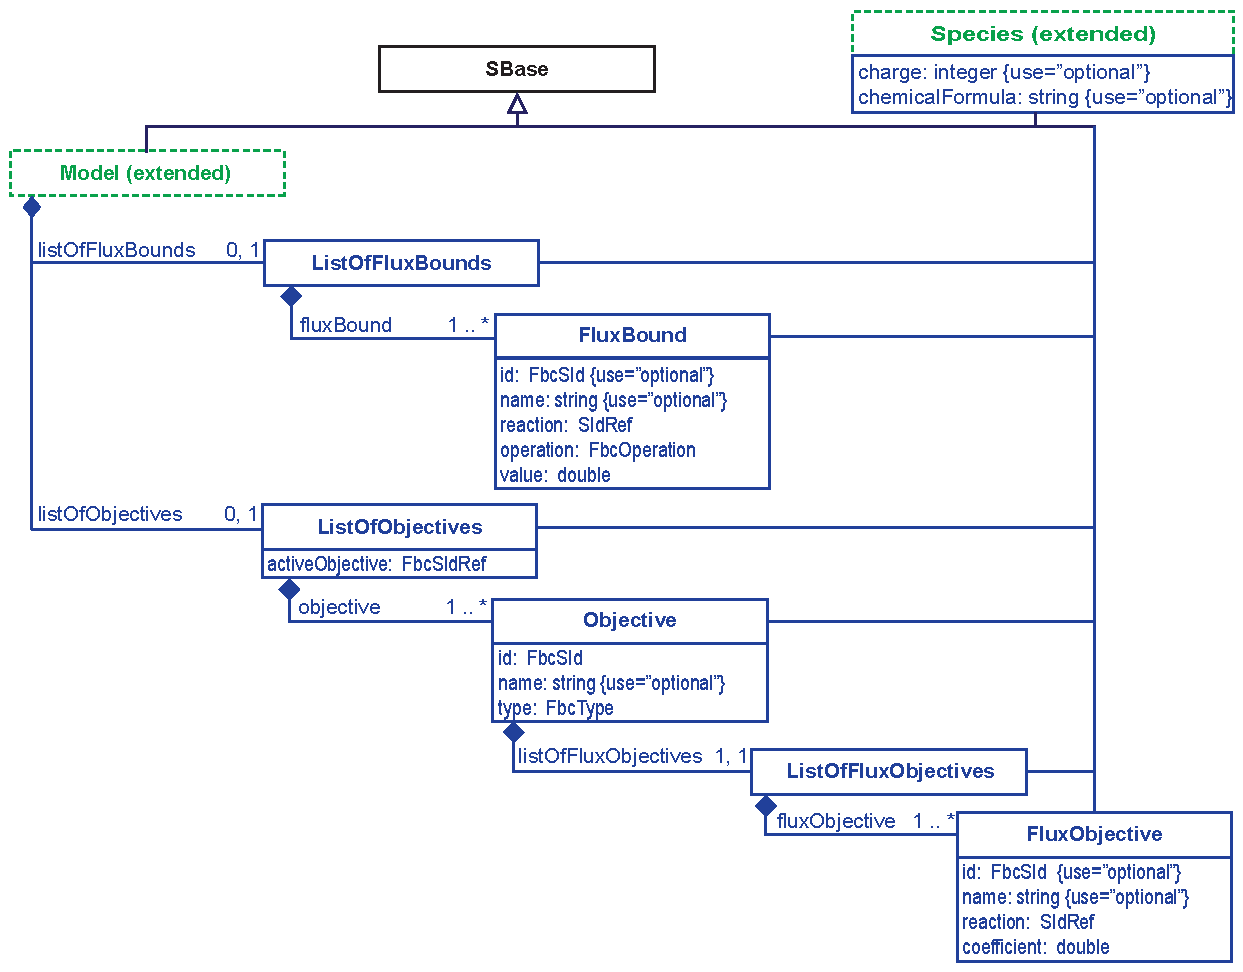
\includegraphics[width=\textwidth]{images/fbc_uml.pdf}\\
  \caption{A UML representation of the \FBCPackage. Derived from \SBase, the \FBC classes inherit support for constructs such as SBML \Notes and \Annotation's. See \ref{conventions} for conventions related to this figure. The individual classes are further discussed in the text.}
  \label{fig:fbc_uml}
\end{figure}

\subsection{Primitive data types}
\label{primtypes}

Section~3.1 of the \sbmlthreecore specification defines a number of primitive
data types and also uses a number of XML Schema 1.0 data types~\citep{biron:2000}.
More specifically we make use of \primtype{integer}, \primtype{double},
\primtype{string}, \primtype{SId} and \primtype{SIdRef}. In addition we make use of
%four new primitives \primtype{FbcSId}, \primtype{FbcSIdRef} as well as
two new primitives: the enumerations \primtype{FbcType} and \primtype{FbcOperation},
see \ref{fig:fbc_uml} for the interrelation between these entities.

The \primtype{SId} type is used as the data type for the identifiers of \FluxBound
(\ref{fluxbound-class}), \FluxObjective (\ref{fluxobjective-class}) and \Objective
(\ref{objective-class}) classes. In the FBC package the \ListOfObjectives has an
attribute of type \primtype{SIdRef} that is used to refer to an `active' \Objective.

%\subsubsection{Type \primtypeNC{FbcSId}}
%\label{primtype-fbcsid}
%
%The type \primtype{FbcSId} is derived from \primtype{SId} (\sbmlthreecore
%specification Section~3.1.7) and has identical syntax. The \primtype{FbcSId}
%type is used as the data type for the identifiers of \FluxBound
%(\ref{fluxbound-class}), \FluxObjective (\ref{fluxobjective-class}) and \Objective (\ref{objective-class}) classes. By
%using a separate identifier type we differentiate them from others defined
%in the \SBML model and thus ensuring data encapsulation.
%The equality of \primtype{FbcSId} values is determined by an exact character sequence match and therefore comparisons of these identifiers must be performed in a case-sensitive manner.

%\subsubsection{Type \primtypeNC{FbcSIdRef}}
%\label{primtype-fbcsidref}
%
%Type \primtype{FbcSIdRef} is used for all attributes that refer to identifiers of type \primtype{FbcSId}.  Derived from \primtype{FbcSId} it has the restriction that the value of an attribute having type \primtype{FbcSIdRef} must match the value of a \primtype{FbcSId} attribute in the current model. In the FBC package the \ListOfObjectives has an attribute of this type that is used to refer to an
%`active' \Objective.

\subsubsection{Type \primtypeNC{FbcType}}
\label{primtype-fbctype}

The \FBCPackage defines a new enumerated type \primtype{FbcType} which
represents the optimization sense of the objective function. It can have one
of the following two values \val{maximize} or \val{minimize}.

\subsubsection{Type \primtypeNC{FbcOperation}}
\label{primtype-fbcoperation}

The \FBCPackage defines a new enumerated type \primtype{FbcOperation} which
represents a boolean operator. It can take only one of the following values:
\val{lessEqual}, \val{greaterEqual} or \val{equal}.
%\val{less}, \val{greater}

\newpage
\subsection{The extended \class{Model} class}
\label{model-class}
\label{listoffluxbounds-class}
\label{listofobjectives-class}

The \SBML \Model class is extended with the addition of two children, i.e. a
\token{listOfFluxBounds} and a \token{listOfObjectives} and a \Model may contain at most one of these lists.

\subsubsection{The \FBC \class{listOfFluxBounds}}

As shown in \ref{fig:fbc_uml} the \ListOfFluxBounds is derived from \SBase
and inherits the attributes \token{metaid} and \token{sboTerm}, as well as
the subcomponents for \Annotation and \Notes. \ListOfFluxBounds must contain
at least one \FluxBound (defined in \ref{fluxbound-class}).

\subsubsection{The \FBC \class{listOfObjectives}}

As shown in \ref{fig:fbc_uml} the \ListOfObjectives is derived from \SBase
and inherits the attributes \token{metaid} and \token{sboTerm}, as well as
the subcomponents for \Annotation and \Notes. Unlike most other \SBML
\textsf{\textbf{ListOf\rule{0.15in}{0.5pt}}} classes, \ListOfObjectives
introduces an additional required attribute \token{activeObjective}. The
\ListOfObjectives must contain at least one \Objective (defined in
\ref{objective-class}).

\paragraph{The \token{activeObjective} attribute}
\label{activeObjective-attribute}

This attribute is of type \primtype{SIdRef} and can only refer to the
\token{id} of an existing \Objective. This required attribute exists
so that when multiple \Objective's are included in a single model, the
model will always be well described i.e. there is a single, primary
objective function which defines a single optimum and its associated
solution space.

\subsubsection{A note on units}
\label{fbcunits}
The main unit definitions that should be considered when using the \FBCPackage are the global model definitions of ``extent''  and ``time'' as all \FBC flux related classes (i.e.~\FluxBound and \FluxObjective implicitly attain the same unit as the \Reaction that they reference). More details on units can be found in their respective class definitions.

\subsection{The extended \class{Species} class}
\label{species-class}

The \FBCPackage extends the \sbmlthreecore \Species class with the addition
of two attributes:

\paragraph{The \token{charge} attribute}
The optional attribute \token{charge} which contains a signed
\primtype{integer} referring to the \Species object's charge and is
defined as it was in the \SBML Level 2 Version 1 specification
: \textit{``The optional field charge takes an integer indicating
the charge on the species (in terms of electrons, not the SI unit coulombs).''}

\paragraph{The \token{chemicalFormula} attribute}
\label{chemicalFormula-attribute}
The optional attribute \token{chemicalFormula} containing a
\primtype{string} that represents the \Species objects elemental
composition.
%
\exampleFile{examples/ex_spec_l3.txt}
%
While there are many ways of referring to an elemental composition the purpose of the \token{chemicalFormula} attribute is to allow reaction balancing and validation which is particularly important in constraint based models.

The format of \token{chemicalFormula} must consist only of atomic names (as in the Periodic Table) or user defined compounds either of which take the form of a single capital letter followed by zero or more lowercase letters. Where there is more than a single atom present, this is indicated with an integer. With regards to order (and enhance inter-operability) it is recommended to use the Hill system order \cite{hillsystem, hillwikipedia}.
%
\begin{table}[h!]
  %\centering
  H2O4S\qquad C2H5Br\qquad BrH\\
  C10H12N5O13P3\qquad CH3I\\
  \caption{Examples of chemical formulas written using the Hill System. As described in \ref{chemicalFormula-attribute}}\label{table:hill}
\end{table}
%
Using this notation the number of carbon atoms in a molecule is indicated first, followed by the number of hydrogen atoms and then the number of all other chemical elements in alphabetical order. When the formula contains no carbon; all elements, including hydrogen, are listed alphabetically.
%
\begin{figure}[h!]
  \centering
  % Requires \usepackage{graphicx}
  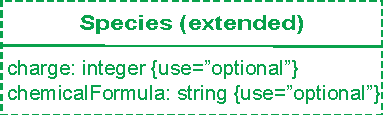
\includegraphics[width=6cm]{images/fbc_uml_species.pdf}\\
  \caption{A UML representation of the extended \SBML \Species class used in
  the \FBCPackage. See \ref{conventions} for conventions related to this
  figure.}
  \label{fig:fbc_uml_species}
\end{figure}

\newpage
\subsection{The \FBC \class{FluxBound} class}
\label{fluxbound-class}

\FluxBound is a new \FBC class derived from \SBML \SBase that inherits
\token{metaid} and \token{sboTerm}, as well as the subcomponents for
\Annotation and \Notes. The purpose of this class is to hold a single
(in)equality that provides the maximum or minimum value that a reaction flux
can obtain at steady state. It implements four attributes.

\paragraph{The \token{id} and \token{name} attributes}
A \FluxBound has two optional attributes: \token{id} an attribute of type
\primtype{SId} and \token{name} an attribute of type \primtype{string}.

\paragraph{The \token{reaction} attribute}
The required \token{reaction} attribute of type \primtype{SIdRef}. This attribute must refer to a \Reaction element defined within the enclosing model.

\paragraph{The \token{operation} attribute}
The \token{operation} attribute contains a value of type
\primtype{FbcOperation} that can take a limited set of boolean operators as
defined in \ref{primtype-fbcoperation}. The \token{operation} attribute
represents a mathematical (in)equality of the form <\token{reaction}>
<\token{operator}> <\token{value}> e.g. R$_{5}$
>= 0, R$_{5}$ <= $\infty$ and R$_{7}$ = 1.0. The mapping between traditional
mathematical symbols and \primtype{FbcOperation} values is as follows:
%
\begin{eqnarray*}
% I'm using \mapsto until I can find the proper symbol - bgoli
\label{fb-operation-enum}
 \nonumber
  <= & \mapsto & \textrm{``}\mathtt{lessEqual}\textrm{''}\\
  >= & \mapsto & \textrm{``}\mathtt{greaterEqual}\textrm{''}\\
  = & \mapsto & \textrm{``}\mathtt{equal}\textrm{''}\\
%  < & \mapsto & \val{less}\\
%  > & \mapsto & \val{greater}
\end{eqnarray*}
%
\paragraph{The \token{value} attribute}
The \token{value} attribute holds a \primtype{double} value representing the
numerical value of the flux bound. This may include an explicitly defined
$\pm\infty$ encoded as a value, e.g. \val{INF}.

\paragraph{Encoding the \FluxBound}
As described in \ref{fluxbound-class} the flux bound represents a
mathematical (in)equality of the form\\ <\token{reaction}> <\token{operator}>
<\token{value}>.\\ In SBML Level~3 Version~1 with \FBC this is encoded as:
%
\exampleFile{examples/ex_fb_fbc.txt}
%
%This example illustrates two things: the encoding of $\infty$ and that care
%should be used when selecting inequalities such as \val{less} or
%\val{greater}. While mathematically there is a difference, this difference
%is only practically relevant when working with rational arithmetic
%(solvers).
%
\begin{figure}[h!]
  \centering
  % Requires \usepackage{graphicx}
  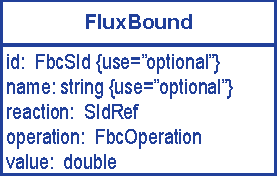
\includegraphics[width=5cm]{images/fbc_uml_fbnd.pdf}\\
  \caption{A UML representation of the \FBCPackage \FluxBound class. See
  \ref{conventions} for conventions related to this figure.}
  \label{fig:fbc_uml_fbnd}
\end{figure}
%
For an example of the how the \FluxBound relates to the description of the underlying mathematical model please see \ref{examples1:fluxbound}.

\paragraph{Units}
The \token{value} defined by the \FluxBound has the units of the \token{reaction} that it refers to i.e.~the globally defined unit of ``extent per time.''

\paragraph{Consistency of flux bounds}

It is possible, and in some cases necessary, to declare more than one
\FluxBound relating to a particular reaction. To allow as much
flexibility to the user as possible, there is no restriction on the
number of flux bounds and the operation specified by each that may be
declared for a given reaction. However, in the case where multiple
flux bounds are declared for one reaction the combined set must not
produce inconsistent values for the upper and lower bounds of the
constraint.

For example

\exampleFile{examples/ex_fb_fbc1.txt}

is obviously inconsistent since it defines \token{R >= 3} and \token{R = 2} - which
cannot be correct.

However

\exampleFile{examples/ex_fb_fbc2.txt}

would be fine since, whilst the information is essentially repeated, \token{R >= 3}
and \token{R = 3} produce the consistent result that \token{R = 3}.



\paragraph{Reactions with undefined flux bounds}
In the spirit of \sbmlthreecore the \FBCPackage does not define any default values for any element. However, in the case of a reaction with no defined flux bounds it is possible to infer this information from the reaction reversibility. In this case: irreversible reactions should be considered to be positive, $0 <= J <= \infty$ and reversible ones free/unbound, $-\infty <= J <= \infty$.

Similarly, there is also the potential for a bound to ``seemingly'' conflict with the reaction that it bounds' reversibility, e.g. a reaction is irreversible but has bounds $-\infty <= J <= \infty$. In the context of this package, flux bounds should be considered authoritative. This follows from the fact that a \FluxBound can enforce an irreversible reaction, by restricting the flux ($0 <= J <= \infty$), as well as a reversible reaction ($-\infty <= J <= \infty$). It is left to the software implementation to deal with any obvious inconsistencies.


\subsection{The \FBC \class{Objective} class}
\label{objective-class}
\label{listoffluxobjectives-class}

The \FBC \Objective class is derived from \SBML \SBase and inherits
\token{metaid} and \token{sboTerm}, as well as the subcomponents for
\Annotation and \Notes. An integral component in a complete description
of a steady-state model is the so-called `objective function' which generally
consist of a linear combination of model variables (fluxes) and a sense
(direction). In the \FBC package this concept is succinctly captured in the
\Objective class.

\paragraph{The \token{id} and \token{name} attributes}
An \Objective has a required attribute \token{id} of type
\primtype{SId} and an optional attribute \token{name} of type \primtype{string}.

\paragraph{The \token{type} attribute}
The required \token{type} attribute contains an \primtype{FbcType} type
which represents the sense of the optimality constraint and can take one of
two values:
\begin{eqnarray*}
% I'm using \mapsto until I can find the proper symbol - bgoli
\label{obj-type-enum}
 \nonumber
  maximize & \mapsto & \textrm{``}\mathtt{maximize}\textrm{''}\\
  minimize & \mapsto & \textrm{``}\mathtt{minimize}\textrm{''}
\end{eqnarray*}

\paragraph{The \token{listOfFluxObjectives} element}
The element \token{listOfFluxObjectives} which contains a
\ListOfFluxObjectives is derived from and functions like a typical \SBML
\textsf{\textbf{ListOf\rule{0.15in}{0.5pt}}} class with the restriction that it
must contain one or more elements of type \FluxObjective (see \ref{fluxobjective-class}).
This implies that if an \Objective is defined there should be at least
one \FluxObjective contained in a \ListOfFluxObjectives.
% bgoli: to me this makes sense but are there other examples of this in SBML or is everything always optional

\begin{figure}[h]
  \centering
  % Requires \usepackage{graphicx}
  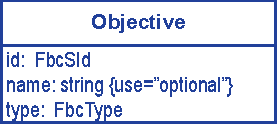
\includegraphics[width=5cm]{images/fbc_uml_obj.pdf}\\
  \caption{A UML representation of the \FBCPackage \Objective class. See
  \ref{conventions} for conventions related to this figure.}
  \label{fig:fbc_uml_obj}
\end{figure}

\paragraph{Encoding the \Objective}
The \FBCPackage allows for the definition of multiple model objectives with
one being designated as active (see \ref{objective-class}) as illustrated in
this example:
%
\exampleFile{examples/ex_objf_fbc.txt}
%
Note how both \Objective instances differ in \token{type} and each contains
different set of \class{FluxObjectives} (see \ref{fluxobjective-class}).
For an example of the how the \Objective relates to the description of the underlying mathematical model please see \ref{examples1:objfunc}.

\subsection{The \FBC \class{FluxObjective} class}
\label{fluxobjective-class}

The \FBC \FluxObjective class is derived from \SBML \SBase and inherits
\token{metaid} and \token{sboTerm}, as well as the subcomponents for
\Annotation and \Notes.

The \FluxObjective class is a relatively simple container for a model
variable weighted by a signed linear coefficient.

\paragraph{The \token{id} and \token{name} attributes}
A \FluxObjective has two optional attributes: \token{id} an attribute of type \primtype{SId} and \token{name} an attribute of type \primtype{string}.

\paragraph{The \token{reaction} and \token{coefficient} attributes}
The required \token{reaction} is of type \primtype{SIdRef} and is restricted to refer only to a \Reaction while the \token{coefficient} attribute holds a \primtype{double} referring to the coefficient that this \FluxObjective takes in the enclosing \Objective. For example the objective \texttt{ Maximize: 1 R1 + 2 R2} would be encoded as
%
\exampleFile{examples/ex_fluxobj_fbc.txt}
%
\begin{figure}[h]
  \centering
  % Requires \usepackage{graphicx}
  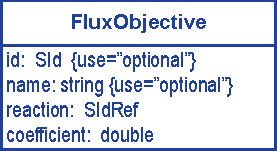
\includegraphics[width=5cm]{images/fbc_uml_fobj.pdf}\\
  \caption{A UML representation of the \FBCPackage \FluxObjective class. See
  \ref{conventions} for conventions related to this figure.}
  \label{fig:fbc_uml_fobj}
\end{figure}

\paragraph{Units}
As described above the \FluxObjective defined here as $n\cdot J$ where the \token{coefficient} ($n$) is dimensionless and the \token{value} ($J$) takes the units of the \token{reaction} flux i.e.~``extent per time''. Therefore, the \FluxObjective ($n\cdot J$)  has the unit ``extent per time'' where the units of reaction ``extent'' and ``time'' are defined globally.



% -*- TeX-master: "sbml-level-3-version-2-core"; fill-column: 66 -*-
% $Id: examples.tex 12140 2010-10-06 05:00:16Z mhucka $
% $HeadURL: https://svn.code.sourceforge.net/p/sbml/code/trunk/specifications/sbml-level-3/version-1/core/spec/examples.tex $
% ----------------------------------------------------------------

% Macros used in this section to provide common typesetting styles.

\newcommand{\species}[1]{\ensuremath{#1}\xspace}
\newcommand{\concent}[1]{\ensuremath{[#1\mkern1mu]}\xspace}
\newcommand{\unit}[1]   {\text{#1}\xspace}

\newcommand{\graybox}[1]{\colorbox[gray]{.85}{#1}}


\section{Example models expressed in XML using SBML}
\label{sec:xml-rep}
\label{sec:examples}

In this section, we present several examples of complete models
encoded in XML using SBML Level~3.


%-----------------------------------------------------------------------------
\subsection{A simple example application of SBML}
\label{sec:modeleg}
%-----------------------------------------------------------------------------

\newcommand{\kon} {\ensuremath{k_\text{on}}\xspace}
\newcommand{\koff}{\ensuremath{k_\text{off}}\xspace}
\newcommand{\kcat}{\ensuremath{k_\text{cat}}\xspace}

Consider the following representation of an enzymatic reaction:
\begin{center}
  \ce{\species{E} + \species{S} <=>[\kon][\koff] \species{ES} ->[\kcat] \species{E} + \species{P}}
\end{center}
In our model, we use the following initial species amounts:
\begin{larray*}
  \species{E}  &=& 5 \cdot 10^{-21} \; \unit{mole} \\
  \species{S}  &=& 10^{-20} \; \unit{mole} \\
  \species{P}  &=& 0 \; \unit{mole} \\ 
  \species{ES} &=& 0 \; \unit{mole}
\end{larray*}
Note that the species quantities are initialized in terms of
substance amounts rather than concentrations.  We also define the
following values for the kinetic constants:
\begin{larray*}
  \kon  &=& 1\:000\:000 \; \unit{litre} \; \unit{mole}^{\,-1} \; \unit{second}^{\,-1}\\
  \koff &=& 0.2 \; \unit{second}^{\,-1}\\
  \kcat &=& 0.1 \; \unit{second}^{\,-1}
\end{larray*}
We place everything in a single compartment we call ``comp'' whose
volume is $10^{-14}$ litres.  The following is a minimal but
complete SBML document encoding this model:

\sbmlexample{enzymekinetics.xml}

The model features local parameter definitions in each reaction.
In this case, the three parameters (\token{kon}, \token{koff},
\token{kcat}) all have unique identifiers and they could also have
just as easily been declared global parameters.  Local parameters
frequently become more useful in larger models, where it may
become tedious to assign unique identifiers for all the different
parameters.

The example above also demonstrates the use of unit specifications
throughout the model.  The \token{model} components define the
units of kinetic laws as being \unit{mole}/\unit{second} by virtue
of the values of the attributes \token{extentUnits} and
\token{timeUnits}.  In the rest of the model, species, parameters
and compartments are defined with appropriate units so that the
mathematical formulas inside the \token{kineticLaw} elements work
out to be \unit{mole}/\unit{second}.


%-----------------------------------------------------------------------------
\subsection{A simple example using the \token{conversionFactor} attribute}
\label{sec:eg:conversionfactor}
%-----------------------------------------------------------------------------

This example involves the same enzymatic reaction as in the
example of Section~\ref{sec:modeleg}:
\begin{center}
  \ce{\species{E} + \species{S} <=>[\kon][\koff] \species{ES} ->[\kcat] \species{E} + \species{P}}
\end{center}
In this new version of the model, we deliberately define the
species with different units from the unit of reaction extent in
the model.  This leads to two illustrative problems: (1) the
reaction rate expressions must be changed in order to reconcile
the differences between the species units and the unit of reaction
extent in the model, and (2) the formulas constructed for species'
rate-of-change equations must use conversion factors to reconcile
the differences between the units of the reaction rate expressions
and the units in which the species quantities are measured.

We begin with the following new \Species object definitions:
\begin{larray*}
  \species{E}   &=& 5 \cdot 10^{-18}\; \unit{millimole} \\
  \species{S}   &=& 10^{-17}\; \unit{millimole} \\
  \species{P}   &=& 0\; \unit{gram} \\
  \species{ES}  &=& 0\; \unit{millimole}
\end{larray*}
We keep the units of extent and time in the model the same as in
Example~\ref{sec:modeleg}; that is, the overall unit of extent in
the model is \unit{mole} and the unit of time is \unit{second},
set by assigning appropriate values to the attributes
\token{extentUnits} and \token{timeUnits}, respectively, on the
\Model object definition.  The differences between these and the
units of the species means that we have to adjust the reaction
rate expressions from their original versions in the model.  In
what follows, we illustrate one approach to doing so, and in
Section~\ref{sec:eg:conversionfactor2} we illustrate a second
approach.  The method in the present section involves changing the
values of the kinetic rate constants in the reaction rate
formulas, while the example of
Section~\ref{sec:eg:conversionfactor2} does not change the kinetic
constants but does require the introduction of additional
parameters.

\newcommand{\veq}    {\ensuremath{v_\text{veq}}\xspace}
\newcommand{\vcat}   {\ensuremath{v_\text{vcat}}\xspace}
\newcommand{\Vcomp}  {\ensuremath{V_\text{comp}}\xspace}
\newcommand{\convE}  {\ensuremath{c_\species{E}}\xspace}
\newcommand{\convS}  {\ensuremath{c_\species{S}}\xspace}
\newcommand{\convP}  {\ensuremath{c_\species{P}}\xspace}
\newcommand{\convES} {\ensuremath{c_{\species{ES}}}\xspace}
\newcommand{\konnew} {\ensuremath{k_\text{on}^{*}}\xspace}
\newcommand{\koffnew}{\ensuremath{k_\text{off}^{*}}\xspace}
\newcommand{\kcatnew}{\ensuremath{k_\text{cat}^{*}}\xspace}

The reaction rate formulas (\ie the formulas in the \token{math}
elements of \KineticLaw objects) were previously
\begin{larray}
  \label{eq:v1}
  \veq  &=& \Vcomp \cdot (\kon \cdot \concent{E} \cdot \concent{S} - \koff \cdot \concent{ES})\\
  \label{eq:v2}
  \vcat &=& \Vcomp \cdot \kcat \cdot \concent{ES}
\end{larray}
where \Vcomp stands for the size of compartment \val{comp} in the
SBML model.  Recalling the values of the parameters \kon, \koff,
and \kcat,
\begin{larray*}
  \kon  &=& 1\:000\:000 \; \unit{litre} \; \unit{mole}^{\,-1} \; \unit{second}^{\,-1}\\
  \koff &=& 0.2 \; \unit{second}^{\,-1}\\
  \kcat &=& 0.1 \; \unit{second}^{\,-1}
\end{larray*}
it becomes clear that, with the values of \species{E}, \species{S}
and \species{ES} all in \unit{millimoles}, Equations~\ref{eq:v1}
and~\ref{eq:v2} no longer lead to units of
\unit{mole}/\unit{second} for the reaction rates.  To compensate,
we change the values of the constants \kon, \koff, and \kcat using
the following simple transformations:
\begin{larray*}
  \konnew = & \kon \cdot \left( \dfrac{1 \; \unit{mole}}{1000 \; \unit{millimoles}} \right)^{2}
  & = 1 \; \unit{litre} \; \unit{mole} \; \unit{millimole}^{-2} \; \unit{second}^{\,-1} \\[4pt]
  \koffnew = & \koff \cdot \dfrac{1 \; \unit{mole}}{1000 \; \unit{millimoles}}
  & = 0.0002 \, \unit{mole} \; \unit{millimole}^{-1} \; \unit{second}^{\,-1} \\[4pt]
  \kcatnew = & \kcat \cdot \dfrac{1 \; \unit{mole}}{1000 \; \unit{millimoles}}
  & = 0.0001 \, \unit{mole} \; \unit{millimole}^{-1} \; \unit{second}^{\,-1}
\end{larray*}\vspace*{0.2ex}
The ``\unit{mole}/\unit{millimole}'' portion of the units are
admittedly unconventional for mass-action kinetic rate constants.
They are unlikely to correspond to values found in textbooks or
databases.  The logic of this approach is that in an actual
experimental situation, with the units of the species as given in
the model (presumably representing how the species are being
measured), the kinetic rate constants are likely to be measured in
terms of the units above.  However, if that is not the case, then
the approach of Section~\ref{sec:eg:conversionfactor2} may be more
appropriate.

\newcommand{\nS}{\ensuremath{n_{\mkern-1muS}}\xspace}
\newcommand{\nP}{\ensuremath{n_{\mkern-1muP}}\xspace}

Taking these new \konnew, \koffnew and \kcatnew parameters and
replacing the original parameters in the reaction rate equations
finally leads to the following:
\begin{larray}
  \label{eq:veq-star}
  \veq  &=& \Vcomp \cdot (\konnew \cdot \concent{E} \cdot \concent{S} - \koffnew \cdot \concent{ES})\\
  \label{eq:vcat-star}
  \vcat &=& \Vcomp \cdot \kcatnew \cdot \concent{ES}
\end{larray}
Next, we turn to the rates-of-change equations for the species.
There are two cases: species \species{S}, whose unit of substance
is \unit{millimole}, and species \species{P}, whose unit of
substance is \unit{gram}.  We use SBML Level~3's conversion factor
mechanism to effectuate the necessary transformations, following
the guidelines described in Section~\ref{sec:about-kinetic-laws}.
In the model text below, we define a default conversion factor by
setting the value of the \Model object's \token{conversionFactor}
attribute to a parameter whose values is
\begin{linenomath}
  \begin{equation*}
    \dfrac{1000 \; \unit{millimole}}{1 \; \unit{mole}}
  \end{equation*}
\end{linenomath}
Let \csg stand for the \Model object's \token{conversionFactor}
attribute with the value above.  The rate-of-change equation for
\species{S} is the following:
\begin{linenomath}
  \begin{equation}\label{eq:dns}
    \dfrac{d \nS}{d t} = - \csg \cdot \graybox{$\Vcomp \cdot
    (\konnew \cdot \concent{E} \cdot \concent{S} - \koffnew \cdot \concent{ES})$}
  \end{equation}
\end{linenomath}
The portion inside the gray box in Equation~\ref{eq:dns} is simply
Equation~\ref{eq:veq-star}, and its value will have the unit
mole/second.  Multiplying this by \csg will produce a result in
millimole/second.  The stoichiometry of species \species{S} in the
reaction is \val{1}, but it is a reactant, thus the need for the
negative sign.

For species \species{P}, we need a different conversion factor, to
convert between the units of \unit{gram} and \unit{mole}.  We
accomplish this by setting a value for the \Species object's
\token{conversionFactor} attribute.  By virtue of being defined on
the \Species object for \species{P}, this conversion factor value
overrides the global value defined on the \Model object.  Let
\convP represent this conversion factor.  The equation for the
rate-of-change of \species{P} is the following:
\begin{linenomath}
  \begin{equation}\label{eq:dnp}
    \dfrac{d \nP}{d t} = \convP \cdot \graybox{$\Vcomp \cdot \kcatnew \cdot \concent{ES}$}
  \end{equation}
\end{linenomath}
The portion inside the gray box in Equation~\ref{eq:dnp} is simply
Equation~\ref{eq:vcat-star}, with a value in mole/second.
Multiplying by the conversion factor \val{convertToGram} defined
in the model below will yield gram/second.  The species
\species{P} is a product, and its stoichiometry is \val{1}; thus,
the right-hand side has a positive sign.

The following is the SBML encoding of this model:

\sbmlexample{conversionfactor1.xml}


%-----------------------------------------------------------------------------
\subsection{An alternative formulation of the \token{conversionFactor} example}
\label{sec:eg:conversionfactor2}
%-----------------------------------------------------------------------------

Here we present an alternative formulation of the model from the
previous section.  Once again, it involves the same enzymatic
reaction as in the example of Section~\ref{sec:modeleg}:
\begin{center}
  \ce{\species{E} + \species{S} <=>[\kon][\koff] \species{ES} ->[\kcat] \species{E} + \species{P}}
\end{center}
As in Section~\ref{sec:eg:conversionfactor}, we define the overall
unit of extent on the model to be \unit{mole} and the unit of time
to be \unit{second}; this means the unit of reaction rates is
\unit{mole}/\unit{second} as before.  We also set the initial
amounts and units as in the previous section:
\begin{larray*}
  \species{E}   &=& 5 \cdot 10^{-18} \; \unit{millimole} \\
  \species{S}   &=& 10^{-17} \; \unit{millimole} \\
  \species{P}   &=& 0 \; \unit{gram} \\
  \species{ES}  &=& 0 \; \unit{millimole}
\end{larray*}
Unlike in the previous section's model, however, here we retain
the values of the kinetic constants as they were originally in the
model of Section~\ref{sec:modeleg}:
\begin{larray*}
  \kon  &=& 1\:000\:000 \; \unit{litre} \; \unit{mole}^{\,-1} \; \unit{second}^{\,-1}\\
  \koff &=& 0.2 \; \unit{second}^{\,-1}\\
  \kcat &=& 0.1 \; \unit{second}^{\,-1}
\end{larray*}
We take a different approach to adjusting the reaction rate
expressions to account for the fact that the concentrations of the
species as they appear in the \KineticLaw elements are in units of
\unit{millimole}/\unit{litre}, while the unit of reaction extent
is \unit{mole} and reaction rates are in
\unit{mole}/\unit{second}.  Our approach here is to introduce
constants into the reaction rate expressions to convert the
substance units to \unit{mole} and multiply each occurence of a
concentration by that constant.  A separate constant is necessary
for each \Species object appearing in a \KineticLaw object,
although it turns out that in the particular situation under
consideration here, the constants are all identical:
\begin{linenomath}
  \begin{equation*}
      \convE = \convS = \convES = 10^{-3} \; \unit{mole} \; \unit{millimole}^{\,-1}
  \end{equation*}
\end{linenomath}
Applying this approach, the reaction rate equations become the
following:
\begin{larray*}
  \veq  &=& \Vcomp \cdot (\kon \cdot \concent{E} \cdot \convE \cdot \concent{S} \cdot \convS
  - \koff \cdot \concent{ES} \cdot \convES)\\
  \vcat &=& \Vcomp \cdot \kcat \cdot \concent{ES} \cdot \convES
\end{larray*}
where again \Vcomp stands for the size of compartment called
\val{comp} in the SBML model.  We construct the rate-of-change
equations for the each species using the guidelines described in
Section~\ref{sec:about-kinetic-laws}, and in this case, the
equations for species \species{S} and \species{P} are
\begin{larray*}
  \dfrac{d \nS}{d t} &=& - \csg \cdot \Vcomp \cdot
  (\kon \cdot \concent{E} \cdot \convE \cdot \concent{S} \cdot \convS
  - \koff \cdot \concent{ES} \cdot \convES) \\[5pt]
  \dfrac{d \nP}{d t} &=& \convP \cdot \Vcomp \cdot \kcat \cdot \concent{ES} \cdot \convES
\end{larray*}
where again \csg stands for the value of the \Model object's
\token{conversionFactor} attribute and \convP is the value of the
\token{conversionFactor} attribute of the \Species object
definition for \species{P}.

The SBML encoding of this model is given below:

\sbmlexample{conversionfactor2.xml}


%-----------------------------------------------------------------------------
\subsection{Example of a discrete version of a simple dimerization reaction}
\label{sec:discrete-eg}
%-----------------------------------------------------------------------------

\emph{(SBO annotations for this model contributed by Lukas Endler,
  EMBL-EBI, Cambridge, UK.)}

This example illustrates subtle differences between models
formulated for use in a continuous simulation framework (\eg using
differential equations) and those intended for a discrete
simulation framework.  The model shown here is suitable for use
with a discrete stochastic simulation algorithm of the sort
developed by \cite{gillespie:1977}.  In such an approach, species
are described in terms of molecular counts and simulation
proceeds by computing the probability of the time and identity of
the next reaction, then updating the species amounts
appropriately.

The model involves a simple dimerization reaction for a protein
named \species{P}:
\begin{linenomath}
\begin{equation*}
    2 P  \leftrightarrow  P_2
\end{equation*}
\end{linenomath}
The SBML representation is shown below.  There are several notable
points.  First, species \species{P} and \species{P_2} (represented
by \val{P} and \val{P2}, respectively) are declared to be always
in terms of discrete amounts by using the flag
\token{hasOnlySubstanceUnits}=\val{true} on the \Species object
definitions.  This indicates that when the species identifiers
appear in mathematical formulas, their values have units of
\quantity{substance amount}, not \{\quantity{substance
  amount}\}/\quantity{size}.  A second point is that, as a result,
the corresponding \KineticLaw formulas do not need volume
corrections.  In Gillespie's approach, the constants in the rate
expressions (here, $c_1$ and $c_2$, represented in the SBML model
by \token{c1} and \token{c2}, respectively) contain a contribution
from the kinetic constants of the reaction and the size of the
compartment in which the reactions take place.  This is a
convention commonly adopted by stochastic modelers, but is in no
way essential---it is perfectly reasonable to factor volume out of
the rate constants, and in certain situations it may be desirable
to do so (\eg for models having time-varying compartment volume),
but due to the use of substance units, it must be done differently
compared to the deterministic case.  Third, although the reaction
is reversible, it is encoded as two separate irreversible
reactions, one each for the forward and reverse directions, as
averaging over the reactions will affect the stochasticity.
Finally, note that the rate expression for the forward reaction is
a second-order mass-action reaction, but it is the \emph{discrete}
formulation of such a reaction rate~\citep{gillespie:1977}.

\sbmlexample{dimerization.xml}

This example also illustrates the need to provide additional
information in a model so that software tools using different
mathematical frameworks can properly interpret it.  In this case,
a simulation tool designed for continuous ODE-based simulation
would likely misinterpret the model (in particular the reaction
rate formulas), unless it deduced that a discrete stochastic
simulation was intended.  One of the purposes of SBO annotations
(Section~\ref{sec:sboTerm}) is to enable such interpretation
without the need for deduction. However, the interpretation of the
model is essentially the same irrespective of whether the model is
to be simulated in a deterministic or stochastic manner, and a
properly SBML-compliant deterministic simulator will in most cases
correctly simulate the continuous deterministic approximation
of the stochastic model even if it has no stochastic simulation
capability.

\clearpage 

The interpretation of rate laws for stochastic models is similar
to, yet different from, that of deterministic models. Taking the
first reaction as an example, the rate law is $c_1P(P-1)/2$ reaction
events per second. In the continuous deterministic case, the
interpretation of this is that the extent of the reaction in time
$dt$ is $[c_1P(P-1)/2]dt$ (and this leads naturally to the usual ODE
formulation of the model). In the stochastic case, the
interpretation is that the \emph{propensity} (or \emph{rate}, or
\emph{hazard}) of the reaction is $c_1P(P-1)/2$. That is, the
\emph{probability} of a single reaction event occurring in time
$dt$ is $[c_1P(P-1)/2]dt$ (and note that the \emph{expected} extent of
the reaction will be $[c_1P(P-1)/2]dt$). This interpretation leads to a Markov
jump process for the system dynamics, where the inter-event times
are exponentially distributed. Such dynamics can be simulated
using a discrete event simulation algorithm such as the
\emph{Gillespie algorithm}. In this case, the algorithm for
simulating the model can be described as follows:

\begin{enumerate}

\item Initialize $t:=0,\ c_1:=0.00166,\ c_2:=0.2,\ P:=301,\ P_2:=0$

\item Compute $h_1:=c_1P(P-1)/2,\ h_2:=c_2P_2$

\item Compute $h_0=h_1+h_2$

\item Simulate $t'\sim \operatorname{Exp}(h_0)$ and set $t:=t+t'$

\item With probability $h_1/h_0$ set $P:=P-2,\ P_2:=P_2+1$,
  otherwise set $P:=P+2,\ P_2:=P_2-1$.

\item Output $t,\ P,\ P_2$

\item If $t<T_{max}$, return to step 2, otherwise stop.

\end{enumerate}

Although this is a simulation algorithm is a very practical way of
describing how to construct exact realizations of the Markov jump
process corresponding to the discrete stochastic kinetic model, it
is not a concise mathematical description. Such a description can
be provided by writing the model as a time change of a pair of
independent unit Poisson processes. Let $N_1(t)$ and $N_2(t)$ be
the counting functions of these processes, so that for each
$i=1,2$, $t>0$, $N_i(t)\sim \operatorname{Poisson}(t)$. Then,
writing $P(t)$ and $P_2(t)$ for the numbers of molecules of $P$
and $P_2$ at time $t$, respectively, we have that the stochastic process
$\{P(t),P_2(t)\,|\,t>0\}$ satisfies the stochastic integral equation
\begin{larray*}
  P_2(t) &=& N_1\left(\int_0^t
    c_1\frac{P(\tau)[P(\tau)-1]}{2}d\tau\right) - N_2\left(\int_0^t
    c_2 P_2(\tau)d\tau\right) \\[2pt]
  P(t) &=& 301 - 2P_2(t).
\end{larray*}
The above representation is arguably the most useful for
mathematical analysis of the stochastic model; see \cite{ball:2006} for
details. Another popular representation is the so-called chemical
Master equation (CME) for the probability distribution of the possible
states at all times \citep{gillespie:1992}. In this case, since there are
151 possible states of the system (corresponding to the 151
possible values of $P_2$), the CME consists of 151 coupled
ODEs,
\begin{linenomath}
  \begin{equation*}
    \frac{d}{dt}p(P,P_2,t) =
    \left\{
      \begin{array}{ll}
        \displaystyle-\frac{c_1}{2}\times 301\times 299p(301,0,t)+c_2p(299,1,t),
        & P=301,\ P_2=0,\\[10pt]
        \displaystyle\frac{c_1}{2}(P+2)(P+1)p(P+2,P_2-1,t)-\frac{c_1}{2}P(P-1)p(P,P_2,t) & P=301-x,\ P_2=x,\\[5pt]
        \qquad+c_2(P_2+1)p(P-2,P_2+1,t)-c_2P_2p(P,P_2,t),
        & \quad x=1,2,\ldots,149,\\[10pt]
        \displaystyle\frac{c_1}{2}\times 2\times 3p(3,149,t)-c_2\times 150p(1,150,t),
        & P=1,\ P_2=150,
      \end{array}
    \right.
  \end{equation*}
\end{linenomath}
where $p(P,P_2,t)$ denotes the probability that there are $P$
molecules of $P$ and $P_2$ molecules of $P_2$ at time $t$, and the
ODEs are subject to the initial conditions
\begin{linenomath}
  \begin{equation*}
    p(301,0,0)=1,\ p(301-2x,x,0)=0,\ x=1,2,\ldots,150.
  \end{equation*}
\end{linenomath}
See \cite{evans:2008} for further examples of discrete stochastic
kinetic models encoded in SBML and \cite{wilkinson_2006} for an
introduction to discrete stochastic modeling using SBML.



%-----------------------------------------------------------------------------
\subsection{Example involving assignment rules}
\label{apdx:rules-eg}
%-----------------------------------------------------------------------------

This section contains a model that simulates a system containing a
fast reaction.  This model uses rules to express the mathematics
of the fast reaction explicitly rather than using the \token{fast}
attribute on a reaction element.  The system modeled is
\begin{larray*}
  X_0 & \overset{\underrightarrow{k_1 [X_0]}}{}           & S_1 \\[6pt]
  S_1 & \overset{\underleftrightarrow{k_f [S_1] - k_r [S_2]}}{} & S_2 \\[6pt]
  S_2 & \overset{\underrightarrow{k_2 [S_2]}}{}           & X_1
\end{larray*}\vspace*{-1em}
\begin{larray*}
  k_1 = 0.1, \quad k_2 = 0.15, \quad k_f = K_{eq} 10000, \quad k_r = 10000, \quad K_{eq} = 2.5.
\end{larray*}
where $[X_0]$, $[X_1]$, $[S_1]$, and $[S_2]$ are species in
concentration units, and $k_1$, $k_2$, $k_f$, $k_r$, and $K_{eq}$
are parameters.  This system of reactions can be approximated with
the following new system:
\begin{larray*}
  X_0 & \overset{\underrightarrow{k_1 [X_0]}}{} & T \\[6pt]
  T   & \overset{\underrightarrow{k_2 [S_2]}}{} & X_1
\end{larray*}\vspace*{-1.5em}
\begin{larray*}
  [S_1] &=& \dfrac{[T]}{1 + K_{eq}} \\[6pt]
  [S_2] &=& K_{eq} [S_1]
\end{larray*}

where $T$ is a new species.  The following example SBML model
encodes the second system.

\sbmlexample{assignmentrules.xml}


%-----------------------------------------------------------------------------
\subsection{Example involving algebraic rules}
\label{sec:algeraiceg}
%-----------------------------------------------------------------------------

This section contains an example model that contains two
\AlgebraicRule objects that are necessary to determine the values
of two variables within the model.  In this particular case, the
rules cannot be rewritten in terms of \AssignmentRule.  This
example illustrates a more rigorous analysis of the enzymatic
reaction given in the example of Section~\ref{sec:modeleg}.
\begin{center}
  \ce{\species{E} + \species{S} <=>[k1_{\text{on}}][k1_{\text{off}}] \species{ES} ->[k2] \species{E} + \species{P}}
\end{center}
In this example, we describe a quasi-steady-state approximation of
the enzymatic reaction equation shown above.  It is based on two
assumptions.  First, the rate at which the concentration of the
substrate bound enzyme (\concent{ES}) changes is assumed to be
slow compared to the rate of change of concentration of both the
substrate (\concent{S}) and product (\concent{P}).  Second, the
total concentration of the enzyme is assumed to stay constant over
time.  This means we can assume the concentration of \concent{ES}
and \concent{E} are not governed by the reactions, and so some
other equations must be used to determine the values of these
concentrations in order to be able to simulate the model.

Applying the first assumption means that the rate of change of
\concent{ES} should be set to zero:
\begin{linenomath}
\begin{equation*}
  \dfrac{d \concent{ES}}{d t} = k1\sub{on} \cdot \concent{E} \cdot \concent{S}
     - (k1\sub{off} + k2) \cdot \concent{ES} = 0
\end{equation*}
\end{linenomath}

The second assumption can be written as
\begin{linenomath}
\begin{equation*}
  \concent{E\sub{total}} = \concent{E} + \concent{ES}
\end{equation*}
\end{linenomath}
which, after rearranging, becomes
\begin{linenomath}
\begin{equation*}
  \concent{E\sub{total}} - (\concent{E} + \concent{ES}) = 0
\end{equation*}
\end{linenomath}

Thus, we have two algebraic rules that must be applied to
determine the values of \concent{E} and \concent{ES}.  The SBML
encoding of this model is given below.  Note that the species
\species{E} and \species{ES} have their \token{boundaryCondition}
attribute set to \val{true}.  This means that a simulation tool
should not construct equations for them based on the reactions in
the system.  Their values are instead set using the rules in the
model.  Also, the model uses a dummy species
\species{E\sub{total}} with its \token{constant} attribute set to
\val{true}; its role is to assign the total concentration of the
enzyme in the model.  This could just as easily have been done
using a parameter instead of a constant dummy species, but we use
the latter approach as an illustration.

\sbmlexample{twoalgebraicrules.xml}


%-----------------------------------------------------------------------------
\subsection{Example with combinations of
  \token{boundaryCondition} and \token{constant} values on \class{Species}
  with \class{RateRule} objects}
\label{sec:constantspecieseg}
%-----------------------------------------------------------------------------

In this section, we discuss a model that includes four species,
each with a different combination of values for their
\token{boundaryCondition} and \token{constant} attributes.  The
model represents a hypothetical system containing one reaction,
\begin{linenomath}
\begin{equation*}
  \begin{array}{@{}ccc@{}}
    S_1 + S_2 & \overset{\underrightarrow{k_1 [S_1] [S_2] [S_3]}}{} & S_4 \\ \\[-4pt]
  \end{array}
\end{equation*}
\end{linenomath}
where \species{S_3} is a species that catalyzes the conversion of
species \species{S_1} and \species{S_2} into \species{S_4}.
Species \species{S_1} and \species{S_2} are on the boundary of the
system (\ie \species{S_1} and \species{S_2} are reactants but
their values are not determined by kinetic laws).  The value of
\species{S_1} in the system is determined over time by the rate
rule:
\begin{linenomath}
  \begin{equation*}
    \dfrac{d \concent{S_1}}{d t} = k_2
  \end{equation*}
\end{linenomath}
The species \species{S_2} and \species{S_3} are not affected by
the either the reaction or the rate rule, and have the following
initial concentration values:
\begin{linenomath}
  \begin{equation*}
    \concent{S_2} = 1, \quad \concent{S_3} = 2
  \end{equation*}
\end{linenomath}
The values of constant parameters in the system are:
\begin{linenomath}
  \begin{equation*}
    k_1 = 0.5, \quad k_2 = 0.1
  \end{equation*}
\end{linenomath}
and the initial values of varying species are:
\begin{linenomath}
  \begin{equation*}
    \concent{S_1} = 0, \quad \concent{S_4} = 0
  \end{equation*}
\end{linenomath}

The value of \concent{S_1} varies over time and it is on the
boundary, so in the SBML representation, \token{S1} has a
\token{constant} attribute with a value of \val{false} and a
\token{boundaryCondition} attribute with a value of \val{true}.
The value of $\concent{S_2}$ is fixed and it is also on the
boundary, so \token{S2} has a \token{constant} attribute value of
\val{false} and a \token{boundaryCondition} attribute value of
\val{true}.  $\concent{S_3}$ is fixed but not on the boundary, so
the \token{constant} attribute is \val{true} and the
\token{boundaryCondition} attribute is \val{false}.  Finally,
$\concent{S_4}$ is a product whose value is determined by a
kinetic law and therefore in the SBML representation has
\val{false} for both its \token{boundaryCondition} and
\token{constant} attributes.

The following is the SBML rendition of the model shown above:

\sbmlexample{boundarycondition.xml}


%-----------------------------------------------------------------------------
\subsection{Example of translation from a multi-compartmental model to ODEs}
\label{sec:odeeg}
%-----------------------------------------------------------------------------

This section contains a model with two compartments and four
reactions.  The model is derived from Lotka-Volterra, with the
addition of a reversible transport step.  When observed in a
time-course simulation, three of this model's species display
damped oscillations.

\begin{figure}[htb]
  \vspace*{5pt}
  \centering
  \begin{picture}(260,60)
    \put(0,10){\framebox(255,50)[tl]{ cytosol}}
    \put(10,19){\framebox(105,29)[tl]{ nucleus}}
    \put(24,26){$
        X + Y_{1n} \yields^{\cit k\sub{1}} 2\,Y_{1n}
        \eqbm^{\cit K\sub{T}} 2\,Y_{1c} + 2\,Y_2
        \yields^{\cit k\sub{2}} 4\,Y_2 \yields^{\cit k\sub{3}} \emptyset
        $}
  \end{picture}
  \vspace*{-8pt}
  \caption{An example multi-compartmental model.}
  \label{fig:multicomp}
\end{figure}

Figure~\ref{fig:multicomp} illustrates the arrangement of
compartments and reactions in the model
\token{LotkaVolterra\_transport}.  The reaction between the
compartments called \token{cytosol} and \token{nucleus} is a
transport reaction whose mechanisms are not modeled here; in
particular, the reaction does not take place on the membrane
between the compartments, and is modeled here simply as a process
that spans the two three-dimensional compartments.

The text of the SBML representation of the model is shown below,
and it is followed by its complete translation into ordinary
differential equations.  As usual, in this SBML model, the
reaction rate equations in the kinetic laws are in substance per
time units.  The reactions have also been simplified to reduce
common stoichiometric factors in the original system depicted in
Figure~\vref{fig:multicomp}.  The species variables in this SBML
representation are in concentration units; their initial
quantities are declared using the attribute \token{initialAmount}
on the \token{species} definitions, but since the attribute
\token{hasOnlySubstanceUnits} is \emph{not} set to true, the
identifiers of the species represent their concentrations when
those identifiers appear in mathematical expressions elsewhere in
the model.  Note that the species whose identifier is \val{X} is a
boundary condition, as indicated by the attribute
\token{boundaryCondition}=\val{true} in its definition.

\sbmlexample{multicomp.xml}

The ODE translation of this model is as follows.  First, we give
the values of the constant parameters:
\begin{larray*}
  k_1   &=& 2500\; \unit{litre} \; \unit{mole}^{\,-1}\; \unit{second}^{\,-1}\\
  k_2   &=& 2500\; \unit{litre} \; \unit{mole}^{\,-1}\; \unit{second}^{\,-1}\\
  K_3   &=& 25000\; \unit{second}^{\,-1}\\
  K_T   &=& 25000\; \unit{second}^{\,-1}
\end{larray*}
Now on to the initial conditions of the variables.  In the
following, the terms $[X]$, $[Y_{1n}]$, $[Y_{1c}]$, and $[Y_2]$
refer to the species' concentrations.  Note that the corresponding
species identifiers \token{X}, \token{Y\_{1n}}, \token{Y\_{1c}}
and \token{Y\_2} in the model are in concentration units, even
though all the values in the model are initialized in terms of
amounts.  (The reason the species identifiers in the model are
still in concentration units goes back to the meaning of the
\token{hasOnlySubstanceUnits} attribute on a \Species; if the
attribute is set to a value of \val{false}, a species' symbol in a
model is interpreted as a concentration or density regardless of
whether its initial value is set using \token{initialAmount} or
\token{initialConcentration}.)  We use $V_n$ to represent the size
of compartment \val{nucleus} and $V_c$ the size of compartment
\val{cytoplasm}:
\begin{larray*}
  V_n    &=& 1\; \unit{litre}\\
  V_c    &=& 5\; \unit{litre}\\
  X      &=& 1\; \unit{mole}\\
  Y_{1n} &=& 1\; \unit{mole}\\
  Y_{1c} &=& 0\; \unit{mole}\\
  Y_2    &=& 1/5\; \unit{mole}
\end{larray*}
And finally, here are the differential equations:
\begin{linenomath}
  \begin{align*}
    \dfrac{d [X]}{d t}    &= 0 \\[6pt]
    V_n \dfrac{d [Y_{1n}]}{d t} &= k_1 [X] [Y_{1n}] [V_n] - K_T \big([Y_{1n}] - [Y_{1c}]\big) V_c
    && \text{reactions production and transport} \\[6pt]
    V_c \dfrac{d [Y_{1c}]}{d t} &= K_T \big([Y_{1n}] - [Y_{1c}]\big) V_c - k_2 [Y_{1c}] [Y_2] V_c
    && \text{reactions transport and transformation} \\[6pt]
    V_c \dfrac{d [Y_2]}{d t}    &= k_2 [Y_{1c}] [Y_2] V_c - k_3 [Y_2] V_c
    && \text{reactions transformation and degradation}
  \end{align*}
\end{linenomath}
As formulated here, this example assumes constant volumes.  If the
sizes of the compartments \val{cytoplasm} or \val{nucleus} could
change during simulation, then it would be preferable to use a
different approach to constructing the differential equations.  In
this alternative approach, the ODEs would compute substance change
rather than concentration change, and the concentration values
would be computed using separate equations.  This approach is used
in Section~\ref{sec:about-kinetic-laws}.


%-----------------------------------------------------------------------------
\subsection{Example involving function definitions}
\label{sec:functioneg}
%-----------------------------------------------------------------------------

This section contains a model that uses the function definition
feature of SBML.  Consider the following hypothetical system:
\begin{linenomath}
\begin{equation*}
  \begin{array}{@{}ccc@{}}
    S_1 & \overset{\underrightarrow{f([S_1])}}{} & S_2 \\ \\[-4pt]
  \end{array}
\end{equation*}
\end{linenomath}
where
\begin{linenomath}
\begin{equation*}
    f(x) = 2 x
\end{equation*}
\end{linenomath}

The following is the XML document that encodes the model shown
above:

\sbmlexample{functiondef.xml}


%-----------------------------------------------------------------------------
\subsection{Example involving \emph{delay} functions}
\label{sec:delayeg}
%-----------------------------------------------------------------------------

The following is a simple model illustrating the use of $delay$ to
represent a gene that suppresses its own expression.  The model
can be expressed in a single rule:
\begin{linenomath}
\begin{equation*}
  \frac{d [P]}{d t} = \dfrac{ \dfrac{1}{1 + m [P_{delayed}]^q} - [P] }{ \tau }\\
\end{equation*}
\end{linenomath}
\vspace*{-0.5em}
where
\vspace*{-1em}
\begin{larray*}
  [P_\text{delayed}] && \text{is } delay([P], \Delta_t) \text{ or [P] at } t - \Delta_t\\[-2pt]
  [P]           && \text{is protein concentration}\\[-2pt]
  \tau          && \text{is the response time}\\[-2pt]
  m             && \text{is a multiplier or equilibrium constant}\\[-2pt]
  q             && \text{is the Hill coefficient}
\end{larray*}
and the species quantities are in concentration units.
The text of an SBML encoding of this model is given below:

\sbmlexample{delay.xml}


%-----------------------------------------------------------------------------
\subsection{Example involving events}
\label{sec:eventeg}
%-----------------------------------------------------------------------------

This section presents a simple model system that demonstrates the
use of events in SBML.  Consider a system with two genes,
$G_1$ and $G_2$.  $G_1$ is initially
on and $G_2$ is initially off.  When turned on, the two
genes lead to the production of two products, $P_1$ and $P_2$,
respectively, at a fixed rate.  When $P_1$ reaches a given
concentration, $G_2$ switches on.  This system can be
represented mathematically as follows:
\begin{linenomath}
\begin{eqnarray*}
  \dfrac{d [P_1]}{d t} & = & k_1 \big([G_1] - [P_1]\big)\\[3pt]
  \dfrac{d [P_2]}{d t} & = & k_2 \big([G_2] - [P_2]\big)\\[0pt]
  [G_2] & = &
    \begin{cases}
      0 & \text{when $[P_1] \leq \tau$},\\
      1 & \text{when $[P_1] > \tau$}.
    \end{cases}
\end{eqnarray*}
\end{linenomath}

The initial values are:
\begin{linenomath}
\begin{equation*}
  [G_1] = 1, \quad [G_2] = 0, \quad \tau = 0.25, \quad P_1 = 0, \quad P_2 = 0, \quad k_1 = k_2 = 1.
\end{equation*}
\end{linenomath}

The SBML Level 3 representation of this is as follows:

\sbmlexample{events.xml}


%-----------------------------------------------------------------------------
\subsection{Example involving two-dimensional compartments}
\label{sec:two-dimensional-eg}
%-----------------------------------------------------------------------------

The following example is a model that uses a two-dimensional
compartment.  It is a fragment of a larger model of calcium
regulation across the plasma membrane of a cell.  The model
includes a calcium influx channel, \val{Ca\_channel}, and a
calcium-extruding PMCA pump, \val{Ca\_Pump}.  It also includes two
cytosolic proteins that buffer calcium via the
\val{CalciumCalbindin\_gt\_BoundCytosol} and
\val{CalciumBuffer\_gt\_BoundCytosol} reactions.  Finally, the
rate expressions in this model do not include explicit factors of
the compartment volumes; instead, the various rate constants are
assumed to include any necessary corrections for volume.

\sbmlexample{twodimensional.xml}


%-----------------------------------------------------------------------------
\subsection{Example of a reaction located at a membrane}
\label{sec:eg:membrane-reaction}
%-----------------------------------------------------------------------------

\label{sec:reaction-membrane-eg}This section describes a model containing
one single enzymatic reaction where substrate and product are located
in the same compartment but the enzyme is localized at the membrane
surrounding the compartment.

\begin{center}
$R$: \ce{S ->[\ensuremath{[E]}] P}
\par\end{center}

The model contains two compartments, a three-dimensional one
called {}``cytosol'' and a two-dimensional one called
{}``membrane'' that is assumed to be the boundary of the cell. The
reaction $R$ has a substrate $S$ and a product $P$ that are both
located in the cytosol. The enzyme $E$ that catalyzes the
reactions is located at the membrane. The kinetic law of reaction
$R$ is\[ v=A\cdot\frac{k_{cat}\cdot[E]\cdot[S]}{K_{M}+[S]}\] where
$A$ is the area of the membrane (measured in $\mu m^{2}$), $[E]$
is the density of the enzyme on the membrane (in
$\mu\mathrm{mol}~\mu m^{-2}$), $[S]$ is the concentration of the
substrate (in $\mu mol~l^{\,-1}$), $K_{M}$ the Michaelis-Menten
constant (also in $\mu mol~l^{\,-1}$), and $k_{cat}$ the rate
constant (in $min^{-1}$). The units of the result of the kinetic
law are in $\mu mol~min^{-1}$. Since the units for the amounts of
all species ($S$, $P$, and $E$) and for the reaction extent are
the same ($\mu mol$) the model does not require unit conversion
factors.

The kinetic law as it is given here scales correctly for changes
in cytosol volume, membrane area, or enzyme density. This means
that if one of these values is changed (even if it varies during a
simulation) the rate expression remains valid.

The following is the text of the model's SBML representation.

\sbmlexample{membrane.xml}


%-----------------------------------------------------------------------------
\subsection{Example using an event with a non-persistent trigger and a delay}
\label{sec:eg:nonpersistent-trigger}
%-----------------------------------------------------------------------------

This example illustrates the syntax and use of the \Trigger object
on \Event, particularly the \token{persistent} attribute, as well
as the optional \Delay object on \Event.  In the model below, the
event has a trigger expression that tests the value of species
\val{a} in the model, and if the value comes within the range
$0.999 \leq a \leq 1.001$, the event triggers and reassigns the
value of \val{c} after a delay of 3 seconds.

\sbmlexample{persistent-event.xml}

% -*- TeX-master: "main"; fill-column: 72 -*-

\section{Best practices}
\label{best-practices}

In this section, we recommend a number of practices for using and interpreting the various constructs in the \token{dyn} package. Neglecting these recommendations may not render a model invalid, but may reduce the degree of interoperability that can be achieved when sharing it. Hence, we strongly advocate the following practices when using the \sbmlthreedynamic:


%\documentclass{cekarticle}
\usepackage{color}
\usepackage{amsmath}
\usepackage{amssymb}
\usepackage{array}

\begin{document}

%=============================================================================
% Title page
%=============================================================================

\title{Systems Biology Markup Language (SBML) Level 2 Proposal: Miscellaneous Features}

\author{Andrew Finney, Victoria Gor, Eric Mjolsness, Hamid Bolouri}

\authoremail{
\begin{minipage}{\textwidth}\centering
afinney@cds.caltech.edu, gor@aig.jpl.nasa.gov,\\Eric.D.Mjolsness@jpl.nasa.gov, hbolouri@cds.caltech.edu
\end{minipage}}

\maketitlepage

%=============================================================================
\section{Introduction}
\label{sec:introduction}
%=============================================================================

This document describes proposed features for inclusion in
Systems Biology Markup Language (SBML) Level 2. These features do
not address specific requirements that will enable SBML Level 2
to represent biochemical structures and processes but instead
could potentially form a useful foundation for the features
proposed elsewhere for inclusion in SBML Level 2.

This document is not a definition of SBML Level 2 or part of it.
This document simply presents various features which could be
incorporated into SBML Level 2 as the Systems Biology community
wishes.  This document is intended for detailed review by that
community and to provoke alternative proposals.  Throughout this
document issues that the authors believe will require further
discussion have been highlighted.

The features proposed here are:

\begin{itemize}
\item \textbf{Packages} : a mechanism that enables a model to
document what SBML Level 2 features are used within the model.
see section~\ref{sec:features}.
\item \textbf{Conditional Expressions} : conditional operators
in formulas.  see section~\ref{sec:conditional}.
\item \textbf{Functions} : a mechanism for defining new
functions for use in formulas.  see section~\ref{sec:functions}.
\end{itemize}

Section~\ref{sec:example} includes a complete model which uses
all the features described in this proposal.

For brevity the text of this document is with reference to SBML
Level 1~\citep{hucka:2001} i.e. features are described in terms
of changes to SBML Level 1.  This document uses UML diagrams in
the same way except that new features are shown in red.

All types proposed in this document will be derived from the
\texttt{SBase} type.

\section{Minimal Header for SBML Level 2 documents}

We suggest that the minimal header, that SBML level 2 documents will have, is:

\begin{example}
<?xml version="1.0" encoding="UTF-8"?>
<sbml xmlns="http://www.sbml.org/sbml/level2" version="1" level="2">
\end{example}

\section{Packages}
\label{sec:features}

It is unlikely that systems parsing SBML Level 2 will have
functional internal representations of all the features proposed
for Level 2, for example a given simulator might have a
representation of modularity but not of geometric structures. To
enable a parsing system to check whether a given model is within
its scope it's proposed that an SBML document has an optional
list of \texttt{Package} structures that define the features that
are used by the document.  The proposed new UML definition of the SBML
type is shown in figure~\ref{fig:sbml}.

\begin{figure}[h]
  \vspace*{8pt}
  \centering
  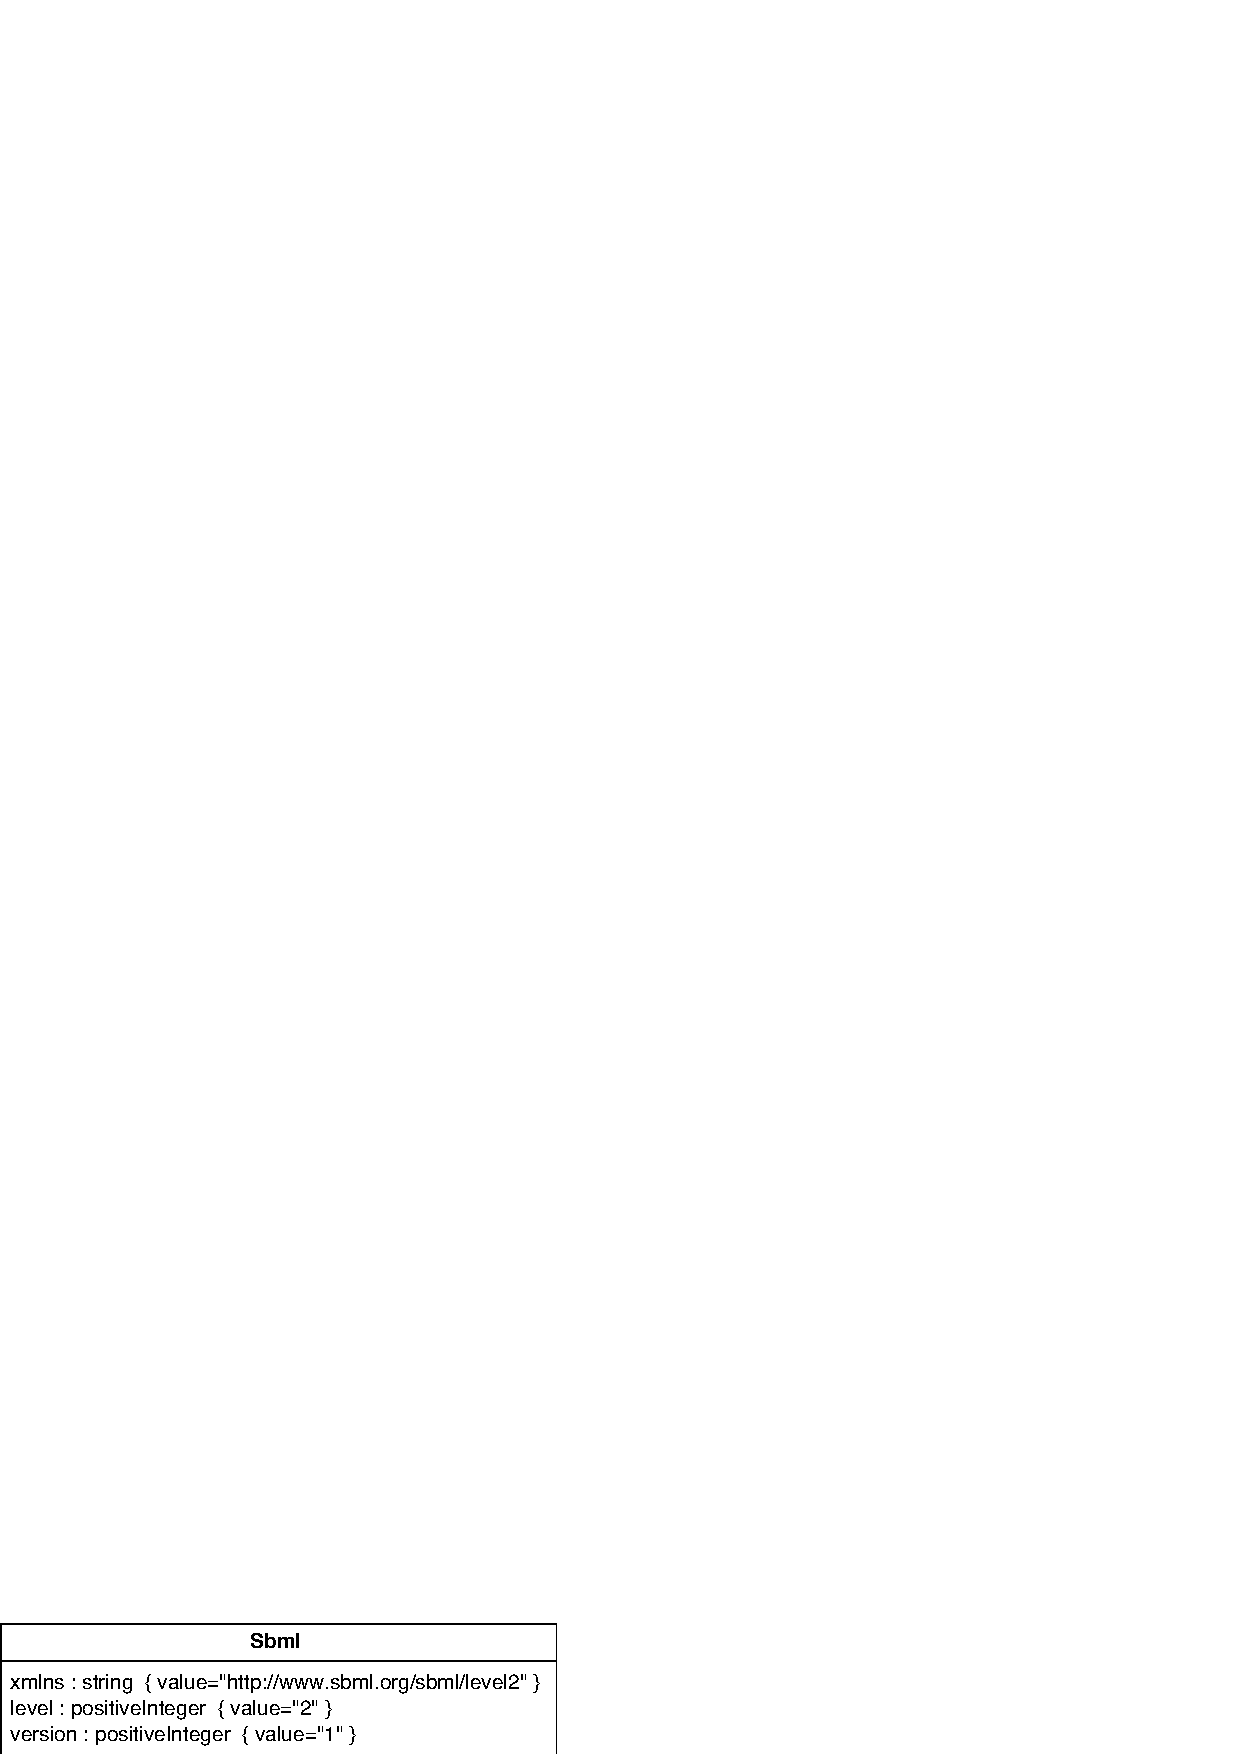
\includegraphics[scale = 0.7]{sbml}
  \caption{The definition of the SBML type}
  \label{fig:sbml}
\end{figure}

In this proposal an \texttt{SBML} structure can optionally
contain a list of \texttt{Features}.  The proposed UML definition of the
\texttt{Feature} type is shown in figure~\ref{fig:feature}.

\begin{figure}[h]
  \vspace*{8pt}
  \centering
  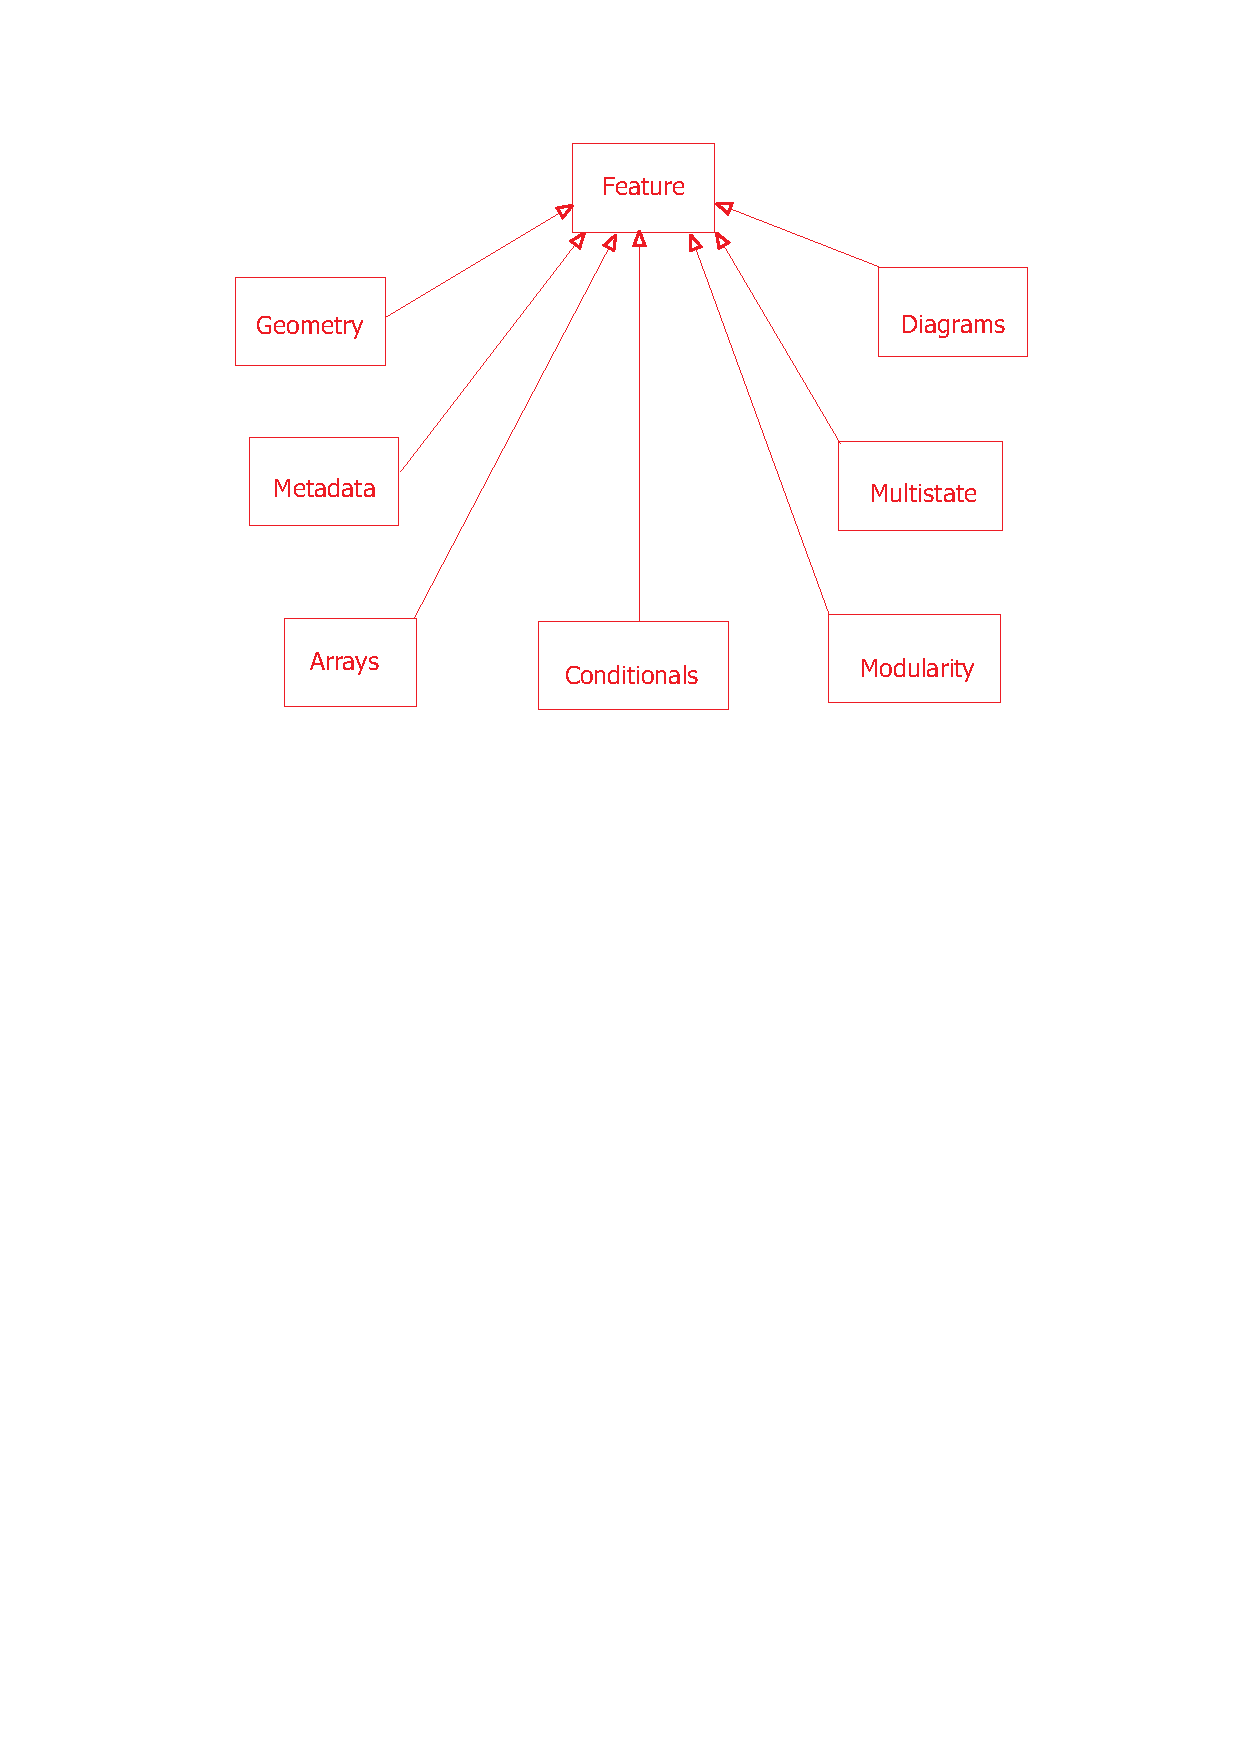
\includegraphics[scale = 0.7]{feature}
  \caption{The definition of the Feature type}
  \label{fig:feature}
\end{figure}

The set of \texttt{Feature} subtypes is very tentative.  It is
proposed that for each of the \texttt{Feature} subtypes there
will be defined a set of SBML elements, numeric expression
functions and numeric expression operators. (These sets will be
defined later).  Each of these sets constitutes a
\emph{package}.  A \emph{package} is used if the document
contains any of the elements or operators in the \emph{package}.

The following proposed list describes the expected scope of each of the
\emph{packages} corresponding to each \texttt{Package} types:
\begin{itemize}
\item \textbf{Geometry}: features needed to support 2D and 3D spatial
models
\item \textbf{Diagrams}: features to store diagrams of models
\item \textbf{Metadata}: features to annotate models, to facilitate
(amongst other things), the linking of model entities to data
external to the models and the systematic storage and retrieval
of models.
\item \textbf{Arrays}: features enabling the inclusion of arrays of
structures/entities in models.  These features would allow a model
to be assembled from many copies of identical parts.  These
features enable the representation of patterns of connection
amongst elements of arrays.
\item \textbf{Multistate}: features enabling the representation of
biochemical entities with a hierarchy of possible states and
applying reactions to those entities with a defined range of
states.  This group is also exploring possible schemes for
representing entities, or complexes, which are graphs of
component entities.
\item \textbf{Modularity}: features enabling the construction of models
from a hierarchy of submodels.  This will allow a given reaction
or process to be modeled at multiple levels of detail.  These
features will allow the construction of models from reusable
components.
\item \textbf{Conditionals}: incorporates conditional operators into
numeric expressions.
\end{itemize}

In this proposal a valid level 2 document would use a subset of
the \emph{packages} that correspond to the \texttt{Package}
elements in the document. The \texttt{Package} lists should not
contain more than one element of a each \texttt{Package} type. An
empty \texttt{Package} list corresponds to the list containing
all possible \texttt{Package} types i.e. the document can contain
any Level 2 operators or elements.  Ideally a document should
contain the smallest non empty valid list of \texttt{Package} structures.

The above list assumes that all systems will be able to support
the functions feature described in section~\ref{sec:functions}.

It is expected that the \texttt{modularity} \emph{package} will allow
more than one \texttt{Model} structure to be contained in an SBML
Level 2 document.  The \texttt{Package} list is a attached to the
\texttt{SBML} structure to ensure that information on the features
used isn't distributed through the document.

\subsection{Example}

The following example of an SBML document header, complying with
this proposal, indicates that the document uses the \texttt{arrays} and
\texttt{conditionals} features.

\begin{example}
<?xml version="1.0" encoding="UTF-8"?>
<sbml xmlns="http://www.sbml.org/sbml/level2" version="1" level="2">
    <listOfFeatures>
        <arrays/>
        <conditionals/>
    </listOfFeatures>
    <model name="cell">
    ...
    </model>
</sbml>
\end{example}

\subsection{Issues}

Some issues that need to be addressed:
\begin{itemize}
\item this concept might be better addressed using separate
namespaces for the different \emph{packages} however this won't
cover the use of operators or functions.  The idea behind this concept is to
enable an event driven parse to halt parsing as soon as the
\texttt{sbml} open tag has been parsed.  As different namespaces
can be added on an ad hoc basis throughout a document, an event
driven parser will have to load the entire document to find all
the namespaces and thus features used in the document.

\item the classification of features will require review at the
end of the development of SBML Level 2.

\item should the \texttt{Conditionals} type be split into
a \texttt{DynamicConditionals} type and a \\
\texttt{StaticConditionals} type? The distinction being between
those conditional expressions where the condition expression
could potentially change during any simulation of the model
(\texttt{DynamicConditionals}) and those that do not
(\texttt{StaticConditionals}).  This information may be an
important criteria by which a simulator will judge whether it can
simulate a model.

\item \texttt{DynamicConditionals} can't be mapped to SBML Level 1.
\end{itemize}

\section{Conditional expressions}
\label{sec:conditional}

This section proposes constructs, for describing discontinuities
via numeric expressions or formula strings.

\subsection{Operators}
Table~\ref{tab:operators} shows a possible extended set of operators that could be
available in SBML Level 2.  New operators are shown in red.  As in
SBML Level 1 these operators work as defined in C except that the
types are always \texttt{double}.  This means that 0 is
interpreted as false and all non zero numbers are interpreted as
true.  The operators \verb|&&| and \verb+||+ short circuit the
evaluation of their second operand depending on the value of the
first operand.

\begin{table}[tbh]
  \vspace*{8pt}
  \begin{center}
    \begin{tabular}{lllcl}
      \toprule
      \textbf{Tokens} & \textbf{Operation} & \textbf{Class} & \textbf{Precedence} & \textbf{Associates} \\
      \midrule
      \emph{name} & symbol reference & operand & 10 & n/a \\
      (\emph{expression}) & expression grouping & operand & 10 & n/a\\
      \emph{f}(\emph{...}) & function call & prefix & 10 & left\\
      \color{red} $!$ & \color{red} logical not & \color{red} unary & \color{red} 9 & \color{red} right\\
      $-$ & negation & unary & 9 & right\\
      \verb|^| & power & binary & 8 & left \\
      $*$ & multiplication & binary & 7 & left\\
      $/$ & division & binary & 7 & left\\
      $+$ & addition & binary & 6 & left\\
      $-$ & subtraction & binary & 6 & left\\
      \color{red} \verb|<| & \color{red} less than & \color{red} binary & \color{red} 5 & \color{red} left\\
      \color{red} \verb|>| & \color{red} greater than & \color{red} binary & \color{red} 5 & \color{red} left\\
      \color{red} \verb|>=| & \color{red} greater than or equal & \color{red} binary & \color{red} 5 & \color{red} left\\
      \color{red} \verb|<=| & \color{red} less than or equal & \color{red} binary & \color{red} 5 & \color{red} left\\
      \color{red} \verb|==| & \color{red} equality & \color{red} binary & \color{red} 4 & \color{red} left\\
      \color{red} \verb|!=| & \color{red} inequality & \color{red} binary & \color{red} 4 & \color{red} left\\
      \color{red} \verb|&&| & \color{red} logical and & \color{red} binary & \color{red} 3 & \color{red} left\\
      \color{red} \verb+||+ & \color{red} logical or & \color{red} binary & \color{red} 2 & \color{red} left \\
      \color{red} \verb|? :| & \color{red} conditional & \color{red} ternary & \color{red} 1 & \color{red} right \color{black} \\
      \bottomrule
    \end{tabular}
  \end{center}
  \caption{A table of the expression operators available in SBML,
    operators proposed in this document are shown in red.  In the
    \textbf{\textrm{Class}} column, ``operand'' implies the construct is an
    operand, ``prefix'' implies the operation is applied to the following
    arguments, ``unary'' implies there is one argument, and ``binary''
    implies there are two arguments.  The values in the
    \textbf{\textrm{Precedence}} column show how the order of different
    types of operation are determined.  For example, the expression $a * b
    + c$ is evaluated as $(a * b) + c$ because the \texttt{*} operator has
    higher precedence.  The \textbf{\textrm{Associates}} column shows how
    the order of similar precedence operations is determined; for example,
    $a - b + c$ is evaluated as $(a - b) + c$ because the $+$ and $-$
    operators are left-associative.  The precedence and associativity rules
    are taken from the C programming language~\protect\citep{harbison:1995},
    except for the symbol \texttt{\^}, which is used in C for a different
    purpose.}
  \label{tab:operators}
\end{table}

\subsection{\texttt{switch} function}

In addition to the new operators described above it is proposed
that an additional `built-in' function \texttt{switch}, is
introduced. This has the form:
\begin{example}
switch(key, match1, result1, ... matchn, resultn, defaultResult);
\end{example}

This function compares \texttt{key} to the values
\texttt{match1...matchn} and returns the \texttt{result} value
immediately following the matching \texttt{match} argument.  If
none of the \texttt{match} arguments are equal to \texttt{key}
then \texttt{switch} returns the \texttt{defaultResult} argument.

The call
\begin{example}
switch(k, m, r, d)
\end{example}
is equivalent to
\begin{example}
(k == m) ? r : d
\end{example}
The call
\begin{example}
switch(k, m1, r1, m2, r2, d)
\end{example}
is equivalent to
\begin{example}
(k == m1) ? r1 : ((k == m2) ? r2 : d)
\end{example}
and so on.

\subsection{Issues}

Given that the function \texttt{switch} and the operators
\texttt{<=}, \texttt{>=} and \texttt{!=} are redundant should
they be incorporated into SBML Level 2?

\section{Functions}
\label{sec:functions}

So as to avoid the continuous revision of SBML, as additional
built-in functions are required, a mechanism is required to allow
the arbitrary definition of new functions in SBML Level 2. This
section proposes such a mechanism.

The proposed UML definition of the \texttt{Model} type is shown in
figure~\ref{fig:model}. (In SBML Level 2 the model type will
probably contain additional optional substructures which are not
shown).  A \texttt{Model} can optionally contain a list of
\texttt{Functions}. Figure~\ref{fig:function} shows the proposed
form of the \texttt{Function} type in UML form.

\begin{figure}[h]
  \vspace*{8pt}
  \centering
  
\includegraphics[scale = 0.7]{model}
  \caption{The definition of the Model type}
  \label{fig:model}
\end{figure}

\begin{figure}[h]
  \vspace*{8pt}
  \centering
  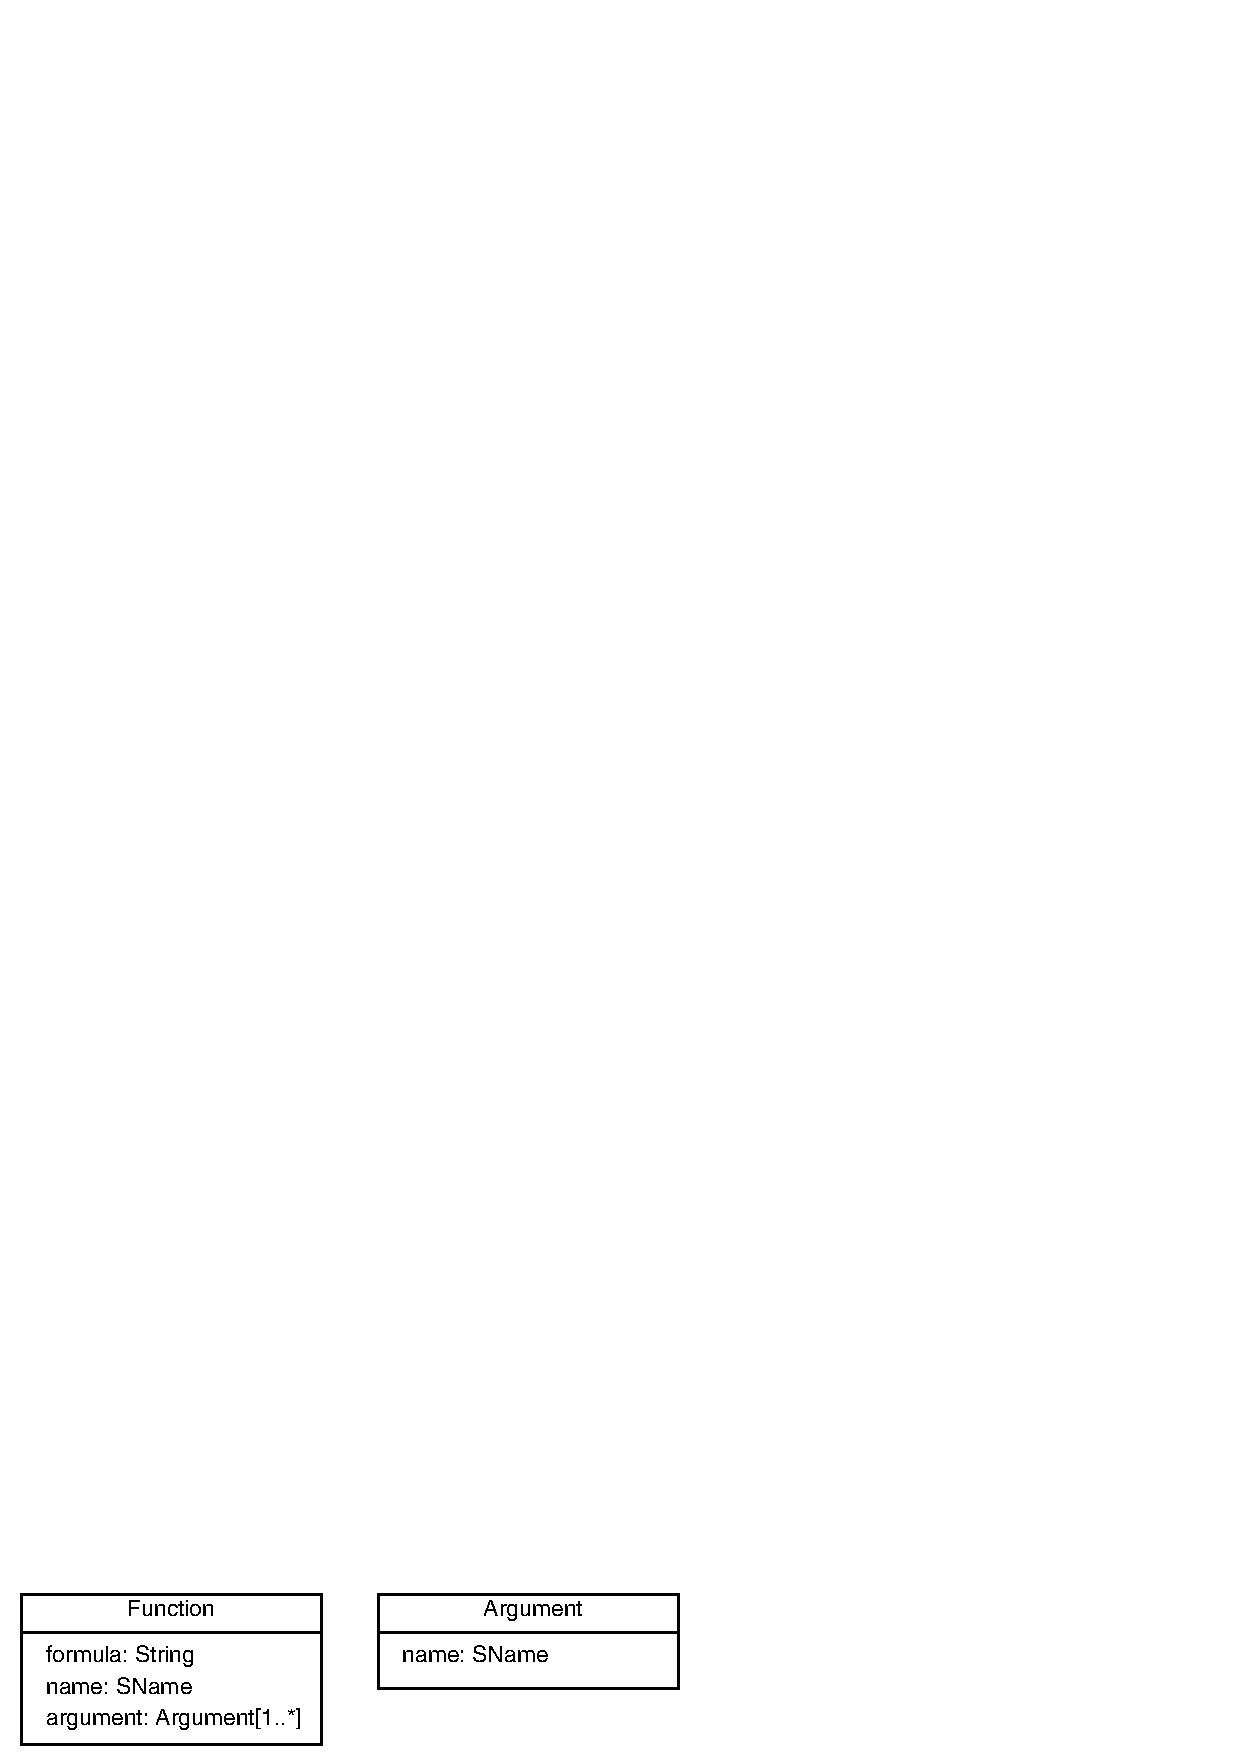
\includegraphics[scale = 0.7]{function}
  \caption{The definition of the Function type}
  \label{fig:function}
\end{figure}

A proposed \texttt{Function} structure consists of the function's name (of
\texttt{SName} type), a formula string and a list of
\texttt{Argument} structures. An \texttt{Argument} structure
simply consists of the argument's name.

A proposed \texttt{Function} structure defines a new function that can be
used in any formula that follows the \texttt{Function} structure.
The only symbols that can be used in the formula string of a
\texttt{Function} structure are the following:
\begin{itemize}
\item \textbf{Arguments:} any of the names given in the \texttt{Argument} list.
\item \textbf{Previously defined functions:} any of the names given in preceding \texttt{Function} structures.
\item \textbf{Built-in functions:} any of the names of built-in functions.
\end{itemize}
These restrictions mean that functions can't be recursive or
mutually recursive thus ensuring that function `calls' can be
expanded in place i.e. models using functions can be mapped to
SBML Level 1.

A \texttt{Function} formula simply returns a \texttt{double}
value.  All the arguments to a function are of type
\texttt{double}.  These functions share the same namespace as
other model-level components, this means that, for example a
function can't have the same name as a specie or a reserved name.

\subsection{Example}

The following is a simple example of a \texttt{Function}
structure in a \texttt{Model} structure:

\begin{example}
<model name="cell">
    <listOfFunctions>
        <function name="pow3" formula="x^3">
            <listOfArguments>
                <argument name="x"/>
            </listOfArguments>
        </function>
    </listOfFunctions>
    ...
</model>
\end{example}

\subsection{Issues}
\begin{itemize}
\item Is the scope of symbols in formulas in functions too restrictive?
\item Do we need to be able to handle objects other than \texttt{double} values?
\end{itemize}

\section{Models with no reactions}

It is proposed that in SBML Level 2 a model can contain no
reactions.  A \texttt{specieConcentrationRule} structures can be
defined to have the same effect as reactions.

\section{Complete Example}
\label{sec:example}

This section contains a complete SBML document which
includes all the proposed features described here.  This model is a
variation on the example model described in~\citet{hucka:2001}.

Consider the following hypothetical branched system:
\begin{equation*}
  \begin{array}{@{}ccc@{}}
    X_0 & \underrightarrow{k_1 pow3(X_0)} & S_1 \\ \\[-4pt]
    S_1 & \underrightarrow{\text{if $S_1 < 1$ then $k_a S_1$ else $k_b S_2$}} & X_1 \\ \\[-4pt]
    S_1 & \underrightarrow{k_3 S_1} & X_2
  \end{array}
\end{equation*}

The following is a XML document that encodes the model shown
above:
\begin{example}
<?xml version="1.0" encoding="UTF-8"?>
<sbml xmlns="http://www.sbml.org/sbml/level2" version="1" level="2">
    <listOfFeatures>
        <conditionals/>
    </listOfFeatures>
    <model name="Branch">
        <notes>
            <body xmlns="http://www.w3.org/1999/xhtml">
                <p>Simple branch system.</p>
                <p>The reaction looks like this:</p>
                <p>reaction-1:   X0 -> S1; k1* pow3(X0);</p>
                <p>reaction-2:   S1 -> X1; S1 < 1 ? k2a*S1 : k2b*S2 ;</p>
                <p>reaction-3:   S1 -> X2; k3*S1;</p>
                <p>where pow3(x) is x^3
            </body>
        </notes>
        <listOfFunctions>
            <function name="pow3" formula="x^3">
                <listOfArguments>
                    <argument name="x"/>
                </listOfArguments>
            </function>
        </listOfFunctions>
        <listOfCompartments>
            <compartment name="compartmentOne" volume="1"/>
        </listOfCompartments>
        <listOfSpecies>
            <specie name="S1" initialAmount="0" compartment="compartmentOne"
                    boundaryCondition="false"/>
            <specie name="X0" initialAmount="0" compartment="compartmentOne"
                    boundaryCondition="true"/>
            <specie name="X1" initialAmount="0" compartment="compartmentOne"
                    boundaryCondition="true"/>
            <specie name="X2" initialAmount="0" compartment="compartmentOne"
                    boundaryCondition="true"/>
        </listOfSpecies>
        <listOfReactions>
            <reaction name="reaction_1" reversible="false">
                <listOfReactants>
                    <specieReference specie="X0" stoichiometry="1"/>
                </listOfReactants>
                <listOfProducts>
                    <specieReference specie="S1" stoichiometry="1"/>
                </listOfProducts>
                <kineticLaw formula="k1 * pow3(X0)">
                    <listOfParameters>
                        <parameter name="k1" value="0"/>
                    </listOfParameters>
                </kineticLaw>
            </reaction>
            <reaction name="reaction_2" reversible="false">
                <listOfReactants>
                    <specieReference specie="S1" stoichiometry="1"/>
                </listOfReactants>
                <listOfProducts>
                    <specieReference specie="X1" stoichiometry="1"/>
                </listOfProducts>
                <kineticLaw formula="S1 < 1 ? ka*S1 : kb*S2">
                    <listOfParameters>
                        <parameter name="ka" value="0"/>
                        <parameter name="kb" value="1"/>
                    </listOfParameters>
                </kineticLaw>
            </reaction>
            <reaction name="reaction_3" reversible="false">
                <listOfReactants>
                    <specieReference specie="S1" stoichiometry="1"/>
                </listOfReactants>
                <listOfProducts>
                    <specieReference specie="X2" stoichiometry="1"/>
                </listOfProducts>
                <kineticLaw formula="k3 * S1">
                    <listOfParameters>
                        <parameter name="k3" value="0"/>
                    </listOfParameters>
                </kineticLaw>
            </reaction>
        </listOfReactions>
    </model>
</sbml>
\end{example}

%=============================================================================
% References
%=============================================================================

\bibliographystyle{apalike}
\bibliography{strings,a,b,c,d,e,f,g,h,i,j,k,l,m,n,o,p,q,r,s,t,u,v,w,x,y,z}
\end{document}


\setcounter{secnumdepth}{2}
\appendix
% -*- TeX-master: "main"; fill-column: 72 -*-

\section{Validation of SBML documents}
\label{apdx-validation}



\setcounter{secnumdepth}{-1}
% -*- TeX-master: "main"; fill-column: 72 -*-

\section{Acknowledgements}

We thank Andrew Finney, Nicolas Le Nov\`{e}re, Stefan Hoops, Martin Ginkel,
Wolfram Leibermeister, Ranjit Randhawa, Jonathan Webb, Frank Bergmann,
Sarah Keating, Sven Sahle, James Schaff, Chris Myers, and the sbml-comp
Package Working Group for prior work, suggestions, and comments that helped
shape the Hierarchical Model Composition package as you see it today.

We also thank with great enthusiasm the financial support of the National
Institutes of Health under grant R01 GM070923 to M. Hucka.


\clearpage
\bibliography{comp}


\end{document}
